%\VignetteIndexEntry{Flexible mediation analysis in R using natural effect models}

\RequirePackage[table]{xcolor}
\documentclass[nojss]{jss}

%%%%%%%%%%%%%%%%%%%%%%%%%%%%%%
%% declarations for jss.cls %%%%%%%%%%%%%%%%%%%%%%%%%%%%%%%%%%%%%%%%%%
%%%%%%%%%%%%%%%%%%%%%%%%%%%%%%

\usepackage[utf8]{inputenc}
\usepackage{amsmath, booktabs, colortbl, nccmath, pifont, tkz-berge}

\defcitealias{iposurl}{IPOS}
\newcommand{\cip}{\mbox{$\perp\!\!\!\perp$}}
\newcounter{dummy}

\allowdisplaybreaks

\author{Johan Steen \\ Ghent University \And
        \hspace{-.5in}Tom Loeys \\ \hspace{-.5in}Ghent University \And
        \hspace{-.7in}Beatrijs Moerkerke \\ \hspace{-.7in}Ghent University \And
        \hspace{-.4in}Stijn Vansteelandt \\ \hspace{-.4in}Ghent University}
\title{\pkg{Medflex}: An \proglang{R} Package for Flexible Mediation Analysis using Natural Effect Models}

%% for pretty printing and a nice hypersummary also set:
\Plainauthor{Johan Steen, Tom Loeys, Beatrijs Moerkerke, Stijn Vansteelandt} %% comma-separated
\Plaintitle{Medflex: an R package for flexible mediation analysis using natural effect models} %% without formatting
\Shorttitle{\pkg{Medflex}: flexible mediation analysis in \proglang{R}} %% a short title (if necessary)

%% an abstract and keywords
\Abstract{
Mediation analysis is routinely adopted by researchers from a wide range of applied disciplines as a statistical tool to disentangle the causal pathways by which an exposure or treatment affects an outcome. The counterfactual framework provides a language for clearly defining path-specific effects of interest and has fostered a principled extension of mediation analysis beyond the context of linear models. This paper describes \pkg{medflex}, an \proglang{R} package that implements some recent developments in mediation analysis embedded within the counterfactual framework. The \pkg{medflex} package offers a set of ready-made functions for fitting natural effect models, a novel class of causal models which directly parameterize the path-specific effects of interest, thereby adding flexibility to existing software packages for mediation analysis, in particular with respect to hypothesis testing and parsimony. In this paper, we give a comprehensive overview of the functionalities of the \pkg{medflex} package.
}
\Keywords{causal inference, mediation analysis, direct effect, indirect effect, natural effect models, \pkg{medflex}, \proglang{R}}
\Plainkeywords{causal inference, mediation analysis, direct effect, indirect effect, natural effect models, medflex, R} %% without formatting
%% at least one keyword must be supplied

\Address{
  Johan Steen\\
  Department of Applied Mathematics, Computer Science and Statistics\\
  Faculty of Sciences\\
  Ghent University\\
  Krijgslaan 281, S9\\
  9000 Gent, Belgium\\
  E-mail: \email{johan.steen@ugent.be}\\
  URL: \url{http://users.ugent.be/~jsteen/}\\
  \\
  Tom Loeys\\
  Department of Data Analysis\\
  Faculty of Psychology and Educational Sciences\\
  Ghent University\\
  Henri Dunantlaan 1\\
  9000 Gent, Belgium\\
  E-mail: \email{tom.loeys@ugent.be}\\
  \\
  Beatrijs Moerkerke\\
  Department of Data Analysis\\
  Faculty of Psychology and Educational Sciences\\
  Ghent University\\
  Henri Dunantlaan 1\\
  9000 Gent, Belgium\\
  E-mail: \email{beatrijs.moerkerke@ugent.be}\\
  \\
  Stijn Vansteelandt\\
  Department of Applied Mathematics, Computer Science and Statistics\\
  Faculty of Sciences\\
  Ghent University\\
  Krijgslaan 281, S9\\
  9000 Gent, Belgium\\
  E-mail: \email{stijn.vansteelandt@ugent.be}
}

\usepackage{Sweave}
\begin{document}
%\SweaveOpts{concordance=TRUE}


%% include your article here, just as usual
%% Note that you should use the \pkg{}, \proglang{} and \code{} commands.

\section[Introduction]{Introduction}
%% Note: If there is markup in \(sub)section, then it has to be escape as above.
Empirical studies often aim at gaining insight into the underlying mechanisms by which an exposure or treatment affects an outcome of interest. Mediation analysis, as popularized in psychology and the social sciences by \cite{Judd1981a} and \cite{Baron1986}, has been widely adopted as a statistical tool to shed light on these mechanisms, by enabling the decomposition of total causal effects into an \textit{indirect} effect through a hypothesized intermediate variable or mediator and the remaining \textit{direct} effect. Although its initial formulations were restricted to the context of linear regression models, several attempts have been made to extend the application of traditional estimators for indirect effects (i.e., product-of-coefficients and difference-in-coefficients estimators) beyond linear settings \citep[e.g.,][]{MacKinnon1993, MacKinnon2007c, Hayes2010, Iacobucci2012}.
However, these extensions lack formal justification and yield effect estimates that are often difficult to interpret \citep[e.g.,][]{Pearl2012}.
\par Recent advances from the causal inference literature \citep[e.g.,][]{Albert2008,Albert2011,Avin2005,Imai2010a,Pearl2001,Pearl2012,Greenland1992,VanderWeele2009b,VanderWeele2010} have furthered these developments and improved both inference and interpretability of direct and indirect effect estimates in nonlinear settings by building on the central notion of counterfactual or potential outcomes. This notion provides a framework that has aided in (i) formally defining direct and indirect effects (in a way that is not tied to a specific statistical model), (ii) describing the conditions required for their identification (unveiling and formalizing often implicitly made causal assumptions) and (iii) assessing the robustness of empirical findings against violations of these identification conditions (i.e., sensitivity analysis). 
\par For instance, \cite{Imai2010b} proposed mediation analysis techniques that can be applied within a larger class of nonlinear models. They implemented these in a user-friendly \proglang{R} package, called \pkg{mediation} (\citealp{R:mediation}; see \citealp{Hicks2011} for a version in \proglang{Stata} \citep{stata} with more limited functionality). More recently, \cite{Valeri2013} reviewed the latest developments in mediation analysis for nonlinear models, focusing on exposure-mediator interactions, and provided \proglang{SAS} \citep{sas} and \proglang{SPSS} \citep{spss} macros, enabling practitioners to easily conduct these methods using well-known commercial packages. Similarly, \cite{Emsley2013} and \cite{Muthen2014} described how direct and indirect effects as defined in the counterfactual framework can be estimated in \proglang{Stata} and via extended types of structural equation models in \proglang{Mplus} \citep{mplus}, respectively.
\par In this paper, we introduce \pkg{medflex} \citep{R:medflex}, an \proglang{R} package that enables flexible estimation of direct and indirect effects while accommodating some of the limitations of other available packages. More specifically, we make use of novel so-called \textit{natural effect models} \citep{Lange2012,Lange2013a,Loeys2013a,Vansteelandt2012}, which directly parameterize the target causal estimands on their most natural scale. This renders formal testing and interpretation more straightforward compared to other approaches as implemented in the aforementioned software applications. The \pkg{medflex} package is freely available from the Comprehensive R Archive Network (CRAN) at \url{http://CRAN.R-project.org/package=medflex} \citep{R:base}.
\par Throughout, the functionalities of the \pkg{medflex} package will be illustrated using data from a survey study that was part of the Interdisciplinary Project for the Optimization of Separation trajectories \citepalias{iposurl}. This large-scale project involved the recruitment of individuals who divorced between March 2008 and March 2009 in four major courts in Flanders. It aimed to improve the quality of life in families during and after the divorce by translating research findings into practical guidelines for separation specialists (such as lawyers, judges, psychologists, welfare workers...) and by promoting evidence-based policy. The corresponding dataset (\code{UPBdata}) is included in the package and involves a subsample of 385 individuals who responded to a battery of questionnaires related to romantic \textit{relationship} characteristics (such as adult attachment style) and \textit{breakup} characteristics (such as breakup initiator status, experiencing negative affectivity and engaging in unwanted pursuit behaviors; UPB) \citep{Smet2012}. Respondents were asked to imagine their former partner as well as possible and to remember how they generally felt in their relationship \textit{before} the breakup when completing the attachment style questionnaire. The mediation hypothesis of interest concerned the question whether the level of emotional distress or negative affectivity experienced \textit{during} the breakup can be regarded as an intermediate mechanism (\textit{M}) through which attachment style towards the ex-partner \textit{before} the breakup (\textit{X}) exerts its influence on displaying UPBs \textit{after} the breakup (\textit{Y}) \citep{Loeys2013a}.
\par In the next section, we briefly introduce the mediation formula \citep{Pearl2001,Pearl2012,Petersen2006,Imai2010a}, which is the predominant vehicle for effect decomposition within the counterfactual framework. Advantages of natural effect models over direct application of the mediation formula will also be discussed in more detail. We then focus on two missing data techniques for fitting these models and demonstrate how these approaches can be implemented in \proglang{R} using the \pkg{medflex} package (Section~\ref{nateff}). Next, we demonstrate how different types of exposure and mediator variables can be dealt with (Section~\ref{types}) and how to assess effect modification of natural effects (i.e., exposure-mediator interactions and moderated mediation) (Section~\ref{modmed}). Tools are provided for calculating and visualizing different causal effects estimates (Section~\ref{tools}) and for estimating population-average natural effects (Section~\ref{popavg}) and natural indirect effects as defined through multiple intermediate pathways jointly (Section~\ref{multmed}). In Section~\ref{weightimp}, we further elaborate on modeling demands and missing data, two aspects that may need
to be taken into consideration by practitioners when choosing between the two main estimation approaches offered by the package. Finally, we conclude with some final remarks and list some extensions of the package which are planned to be implemented in the near future (Section~\ref{concl}).

\section{The mediation formula}
\subsection{Counterfactual outcomes and effect decomposition}
A major appeal of the counterfactual framework is that it enables to decompose the total causal effect into a so-called \textit{natural} direct and \textit{natural} indirect effect, irrespective of the data distribution or scale of the effect. Readers familiar with counterfactual notation, definitions and assumptions for natural direct and indirect effects may wish to skip to section~\ref{medform}. 
\par Let $Y_i(x)$ denote the potential outcome for subject $i$ that had been observed if, possibly contrary to the fact, $i$ had been assigned to treatment (or exposure level) $x$. For a binary exposure (with $X = 1$ for the exposed and $X = 0$ for the unexposed), the individual-level causal effect can then be expressed by comparing $Y_i(1)$ to $Y_i(0)$, whereas the population average total causal effect can be expressed as $\E\{Y(1) - Y(0)\}$. Similarly, direct and indirect effects have been defined in terms of counterfactual outcomes. For instance, the definition of the so-called \textit{controlled} direct effect reflects the traditional notion of measuring the effect of exposure while fixing the mediator $M$ at the same value $m$ for all subjects \citep{Greenland1992}. Using counterfactual notation, this effect can be expressed as
\begin{align*}
\mbox{CDE}(m) &= \E\{Y(1,m) - Y(0,m)\},\\[-\baselineskip]
\hphantom{\mbox{NIE}(1)} &\hphantom{= \E\{Y(1,M(1)) - Y(1,M(0))\},}
\end{align*}
where $Y(x,m)$ denotes the potential outcome that would have been observed under exposure level $x$ and mediator value $m$.
\par \cite{Greenland1992} introduced an alternative definition that invokes so-called \textit{composite} or \textit{nested} counterfactuals, $Y(x,M(x^*))$. For instance, the (pure) natural direct effect 
\begin{align*}
\mbox{NDE}(0) &= \E\{Y(1,M(0)) - Y(0,M(0))\}\\[-\baselineskip]
\hphantom{\mbox{NIE}(1)} &\hphantom{= \E\{Y(1,M(1)) - Y(1,M(0))\},}
\end{align*}
expresses the expected exposure-induced change in outcome when keeping the mediator fixed at the value that had naturally been observed if unexposed. By considering potential intermediate outcomes $M(x^*)$ rather than a fixed mediator value $m$, these authors offered a definition of direct effect that both allows for natural variation in the mediator and provides a complementary operational definition for the indirect effect (which the definition of the controlled direct effect does not). That is, under the composition assumption, which states that $Y(x,M(x)) = Y(x)$ \citep{VanderWeele2009b}, the difference between the average total effect $\E\{Y(1) - Y(0)\}$ and the (pure) natural direct effect yields an expression for the (total) natural indirect effect
\begin{align*}
\mbox{NIE}(1) &= \E\{Y(1,M(1)) - Y(1,M(0))\}.
\end{align*}
This reflects the expected difference in outcome if all subjects were exposed but their mediator value had changed to the value it would take if unexposed.
\par Adopting this counterfactual notation naturally leads to framing causal inference as a missing data problem \citep{Holland1986}: for each subject $i$, only one counterfactual outcome, i.e., $Y_i = Y_i(X_i,M_i(X_i))$, is observed. Consequently, identification of natural effects relies on rather strong causal assumptions. In the context of mediation analysis, the most commonly invoked conditions for identification can be encoded in a causal diagram (such as Figure~\ref{dag1}) interpreted as a non-parametric structural equation model with independent error terms \citep[NPSEM-IE;][]{Pearl2001}. More specifically, upon adjustment for a given set of observed baseline covariates $C$, such model implies certain independencies among variables and potential outcomes (\ref{A1}-\ref{A4}) which have been proposed as sufficient conditions for non-parametric or model-free identification of natural effects. However, this adjustment set $C$ needs to be carefully selected\footnote{\cite{Pearl2001,Pearl2014} offers a weaker set of conditions, which does not require a common set of baseline covariates to deconfound each of the possibly confounded relations, but allows for separate adjustment sets for the exposure-mediator relation on the one hand and the exposure-outcome and mediator-outcome relations on the other hand. This set of conditions is considered weaker, since it allows for identification under certain non-parametric structural equation models with unobserved confounders. Although, theoretically, the natural effect model framework can be shown to easily accommodate separate adjustment sets, this has not been implemented as such in the \pkg{medflex} package. However, as \cite{Imai2014} argue, this weaker set of conditions might be of litte practical relevance since researchers in most settings lack sufficient knowledge about the precise structure of confounding. Nonetheless, the estimation algorithms implemented in the \pkg{mediation} package \citep{R:mediation}, easily allow to specify separate adjustment sets \citep{Imai2014}.}, such that it is deemed sufficient to control for confounding (i) between exposure and outcome, thereby satisfying
\begin{align}
Y(x,m) &\cip X \vert C &&\textrm{for all levels of $x$ and $m$,} \tag{A1}\refstepcounter{dummy}\label{A1}\\[-\baselineskip]
\hphantom{Y(x,m)} &\hphantom{\cip M \vert X=x, C} &&\hphantom{\textrm{for all levels of $x$ and $m$.}}\nonumber
\end{align}
(ii) between exposure and mediator, thereby satisfying
\begin{align}
M(x) &\cip X \vert C &&\textrm{for all levels of $x$,} \tag{A2}\refstepcounter{dummy}\label{A2}\\[-\baselineskip]
\hphantom{Y(x,m)} &\hphantom{\cip M \vert X=x, C} &&\hphantom{\textrm{for all levels of $x$ and $m$.}}\nonumber
\end{align}
and (iii) between mediator and outcome (after adjustment for the exposure), thereby satisfying
\begin{align}
Y(x,m) &\cip M \vert X=x, C &&\textrm{for all levels of $x$ and $m$.} \tag{A3}\refstepcounter{dummy}\label{A3}
\end{align}
In addition to these `no omitted variables' assumptions (\ref{A1}-\ref{A3}), identification requires the further `cross-worlds independence' assumption \citep{Pearl2001}
\begin{align}
Y(x,m) &\cip M(x^*) \vert C &&\textrm{for all levels of $x$, $x^*$ and $m$,} \tag{A4}\refstepcounter{dummy}\label{A4}\\[-\baselineskip]
\hphantom{Y(x,m)} &\hphantom{\cip M \vert X=x, C} &&\hphantom{\textrm{for all levels of $x$ and $m$.}}\nonumber
\end{align}
which is satisfied under a NPSEM-IE when no confounders of the mediator-outcome relationship (whether observed or unobserved) are affected by the exposure (i.e., no intermediate or exposure-induced confounding).
\par Whereas the first two assumptions by definition hold in randomized experiments, the other two assumptions may not.\footnote{Note that \ref{A1} is sufficient for identifying total causal effects, whereas identification of controlled direct effects can be obtained under assumptions \ref{A1} and \ref{A3}.} Although \cite{Judd1981a} initially pointed to its importance, condition~\ref{A3} since has largely been ignored in much of the social sciences literature, as evidenced by many mediation studies not adjusting for confounders of the mediator-outcome relationship. In recent years, however, this issue has been brought back to attention within the social sciences \citep[e.g.,][]{Bullock2010a, MacKinnon2008, Mayer2014}.
\par Condition \ref{A4} is more difficult to grasp intuitively. It is a strong assumption because, in contrast to the other three conditions, it is impossible to design a study that would be able to validate it (\citealt{Robins2010}; although see \citealt{Imai2013a} for a notable attempt).
\par The interested reader can refer to \cite{VanderWeele2009b} for a more detailed and intuitive account of these identification assumptions (or to \citealt{Petersen2006} or  \citealt{Imai2010a} for alternative sets of assumptions).

\subsection{The mediation formula}\label{medform}
The language of counterfactuals has enabled to clearly define causal effects in a more generic, non-parametric way, but has also promoted a more principled approach to estimating these effects than the one offered by the traditional SEM literature from the social sciences, which was mainly entrenched in parametric linear regression.
The main identification result \citep{Pearl2001,Imai2010a}, which \cite{Pearl2012} referred to as the \textit{mediation formula}, has played a pivotal role in this regard. It prescribes estimating the expected value of nested counterfactuals by standardizing predictions from the outcome model corresponding to exposure level $x$ under the mediator distribution corresponding to exposure level $x^*$: $$\E\left\{Y(x,M(x^*))|C\right\} = \sum_m \E(Y|X=x,M=m,C) \Pr(M=m|X=x^*,C).$$  This weighted sum can be calculated based on any type of statistical model and has been shown to yield closed-form expressions for the natural indirect effect that encompass the traditional difference-in-coefficients and product-of-coefficient estimators when confined to strictly linear models \citep[e.g.,][]{VanderWeele2009b, Pearl2012}. However, as soon as moving beyond linear settings, the latter estimators no longer coincide with their corresponding mediation formula expressions and no longer yield readily interpretable causal effect estimates (as formalized in the counterfactual framework).\footnote{\cite{Muthen2014} give an intuitive account for SEM practitioners explaining why the product-of-coefficient estimator fails when applied in nonlinear settings or settings involving exposure-mediator interactions. Nonetheless, the product-of-coefficients method can still be useful for testing the null hypothesis of no indirect effect \citep{VanderWeele2011a,Vansteelandt2012}.}
\par More recently, closed-form expressions for natural direct and indirect effects as defined on both additive and ratio scales have been derived for a limited number of nonlinear scenarios \citep{VanderWeele2009b,VanderWeele2010,Valeri2013}.

\newpage
\subsection{Applying the mediation formula in practice}
Software applications for obtaining closed-form solutions derived from the mediation formula, as well as their corresponding Delta method (or bootstrap) standard errors, have been made available as \proglang{SPSS} and \proglang{SAS} macros \citep{Valeri2013} and as the \proglang{Stata} module \pkg{PARAMED} \citep{Emsley2013}. 
More recently, \cite{Muthen2014} demonstrated how natural effect estimates can be obtained via extended types of structural equation models in \proglang{Mplus}, even in the presence of latent variables. However, such closed-form expressions can often not readily be obtained, for instance when combining a linear model for the mediator and a logistic model for the outcome.
\par \cite{Imai2010a} addressed this issue and instead suggested a more generic approach based on Monte-Carlo integration methods, which they implemented in the \proglang{R} package \pkg{mediation} \citep{R:mediation}.
Whereas its lightweight version in \proglang{Stata} \citep{Hicks2011} and the \proglang{Stata} module \pkg{gformula} \citep{Daniel2011}, which adopts a similar simulation-based approach, are restricted to parametric models, this \proglang{R} package additionally allows to specify semi-parametric models for the mediator and outcome. Despite being computationally intensive, these offer more flexibility than the applications based on a purely analytical approach. In addition, the \pkg{mediation} package offers useful extensions, such as methods for dealing with multiple mediators and treatment noncompliance, while at the same time enabling users to evaluate the robustness of their findings to potential unmeasured confounding in a widely applicable sensitivity analysis.
\par A drawback of direct application of the mediation formula, however, is that combinations of simple models for the mediator and for the outcome often result in complex expressions for natural direct and indirect effects \citep{Lange2012,Vansteelandt2012}. For instance, when using logistic regression models 
\begin{align}
\mbox{logit} \Pr(M=1\vert X,C) &= \alpha_0 + \alpha_1 X + \alpha_2 C\nonumber\\
\mbox{logit} \Pr(Y=1\vert X,M,C) &= \beta_0 + \beta_1 X + \beta_2 M + \beta_3 C \tag{0}\label{0}
\end{align}
for binary mediators and outcomes, the mediation formula yields
\begin{align*}
\Pr(Y(x,M(x^*))=1\vert C) &= \mbox{expit}\left(\beta_0 + \beta_1 x + \beta_2 + \beta_3 C\right)\mbox{expit}\left(\alpha_0 + \alpha_1 x^* + \alpha_2 C\right)\\
&\quad + \mbox{expit}\left(\beta_0 + \beta_1 x + \beta_3 C\right)\left\{1-\mbox{expit}\left(\alpha_0 + \alpha_1 x^* + \alpha_2 C\right)\right\},      
\end{align*}
an expression which depends on exposure and covariate levels in a complicated way. Even though none of the postulated models include interaction terms reflecting effect modification, the corresponding direct and indirect effect estimates will vary with different exposure or covariate levels. This is also illustrated in Figure~\ref{ill}, which depicts estimates for the natural indirect effect odds ratio, as obtained by applying the mediation formula to these models fitted to our example dataset (using a dichotomized version of the mediator and baseline covariates $C$ including gender, age and education level). As pointed out before by \cite{Lange2012} and \cite{Vansteelandt2012}, these convoluted expressions render results difficult to report and hypothesis testing (e.g., testing for moderated mediation) infeasible, as it may turn out impossible to find plausible models for the mediator and outcome that combine into effect expressions that do not depend on covariate levels. In certain cases, this complexity can pose a major impediment to routine application of the mediation formula.
\begin{figure}[t]
\centering
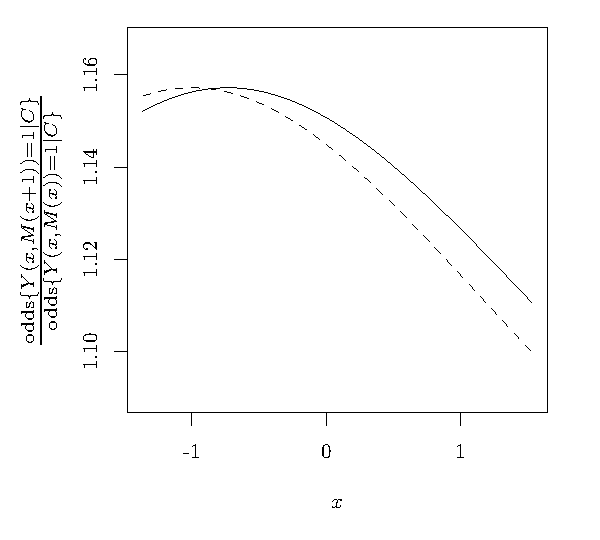
\includegraphics[width=0.7\textwidth]{ill.pdf}
\caption{Estimated (total) natural indirect effect odds ratios corresponding to a one-unit change in anxious attachment level as a function of different reference levels for anxious attachment level $x$ (as obtained through direct application of the mediation formula). These are conditional estimates for 43-year-old men (solid curve) and women (dashed curve) with intermediate education levels.}\label{ill}
\end{figure}
\par Moreover, the \pkg{mediation} package only provides natural effect estimates on the additive scale. This may complicate estimation and inference in nonlinear outcome models, mainly when dealing with continuous exposures or covariates, because of induced nonadditivity. Specifically, because the indirect effect is not encoded by a single parameter, but may take on a different value for each level of $x$, the null hypothesis of no indirect effect over the entire range of exposure levels becomes difficult to test. Similarly, although the \pkg{mediation} package enables users to test for effect modification in nonlinear models (i.e., either treatment-mediator interactions or moderated mediation), these hypothesis tests probe research questions in terms of e.g., risk differences that are tied to pre-specified exposure or covariate levels. A concern is that these levels might, at least in some applications, need to be chosen in a rather arbitrary way \citep{Loeys2013a}.
\par An approach that circumvents the aforementioned complexity but is closely related to application of the mediation formula was recently proposed by \cite{Lange2012} and \cite{Vansteelandt2012}. These authors proposed to directly model the natural effects and introduced a novel class of mean models for nested counterfactuals, which they termed \textit{natural effect models} \citep[also see][for a similar approach]{VanderLaan2008}. This approach is implemented in the \pkg{medflex} package and provides a viable alternative to the aforementioned software applications because
\begin{itemize}
\item it can handle a larger class of parametric models for the mediator and outcome than the software applications that rely on closed-form expressions (refer to Section~\ref{types}),
\item estimates can be expressed on more natural effect scales (i.e., a scale that corresponds to the link-function of the outcome model), thereby avoiding potential induced dependence on exposure or covariate levels characteristic for the additive scale,
\item natural effect models simplify testing since the hypotheses of interest can always be captured by a finite set of model parameters,
\item for the most common types of parametric models robust standard errors (based on the sandwich estimator) are available as an alternative to more computer-intensive bootstrap standard errors.
\end{itemize}
In the next section, we describe this novel class of causal models together with two different approaches that have been suggested in \cite{Lange2012} and \cite{Vansteelandt2012}.

\section{Mediation analysis via natural effect models}\label{nateff}
Natural effect models are conditional mean models for nested counterfactuals $Y(x,M(x^*))$:
\begin{align*}
\E \{ Y(x,M(x^*)) \vert C \} = g^{-1} \{ \beta' W(x,x^*,C) \}
\end{align*}
with $g(\cdot)$ a known link function (e.g., the identity or logit link), $W(x,x^*,C)$ a known vector with components that may depend on $x$, $x^*$ and $C$, and $\beta$ a vector including parameters that encode the natural effects of interest. It can, for instance, easily be inferred that in model
\begin{align*}
\E \{ Y(x,M(x^*)) \vert C \} = \beta_0 + \beta_1 x + \beta_2 x^* + \beta_3 C,
\end{align*}
$\beta_1$ captures the natural direct effect whereas $\beta_2$ captures the natural indirect effect, both corresponding to a one-unit increase in the exposure level. With $g(\cdot)$ the log-link function, for example, the Poisson regression model
\begin{align*}
\log \E \{ Y(x,M(x^*)) \vert C \} = \beta_0 + \beta_1 x + \beta_2 x^* + \beta_3 C,
\end{align*}
enables to quantify the natural direct and indirect effect for count outcomes on a more natural, multiplicative scale. Specifically, in this model, exp($\beta_1$) captures the natural direct effect rate ratio $$\dfrac{\E\{ Y(x+1,M(x)) \vert C \}}{\E\{ Y(x,M(x)) \vert C \}}$$ whereas exp($\beta_2$) captures the natural indirect effect rate ratio $$\dfrac{\E\{ Y(x,M(x+1)) \vert C \}}{\E\{ Y(x,M(x)) \vert C \}},$$ corresponding to a one-unit increase in exposure level. Since each of the effects or quantities of interest are encoded by parameters indexing the natural effect model, the aforementioned limitations related to direct application of the mediation formula can be overcome. As will be illustrated, this facilitates interpretation and hypothesis testing in nonlinear settings.

\newpage
\subsection[]{Fitting natural effect models}
\begin{figure}[b]
  \small
  \centering
  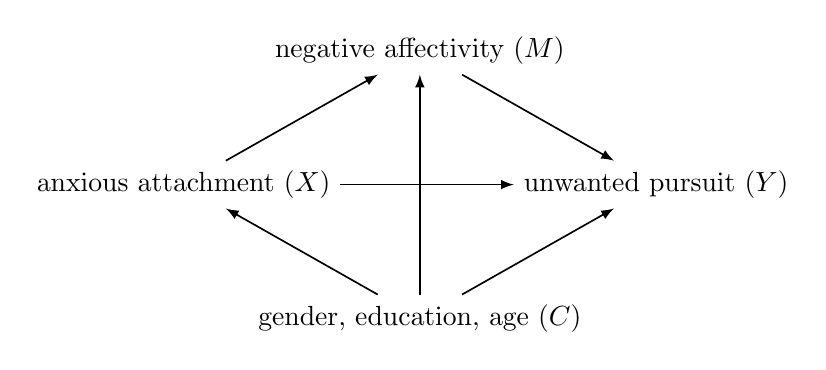
\begin{tikzpicture}[>=latex,semithick]
\node[] (x) at (0, 0)   {anxious attachment ($X$)};
\node[] (m) at (3, 1.7)   {negative affectivity ($M$)};
\node[] (y) at (6, 0)   {unwanted pursuit ($Y$)};
\node[] (c) at (3, -1.7) {gender, education, age ($C$)};
\path[->] (c) edge node [above left] {} (x);
\path[->] (c) edge node [above left] {} (m);
\path[->] (c) edge node [above left] {} (y);
\path[->] (x) edge node [above left] {} (m);
\path[->] (m) edge node [above right] {} (y);
\path[->] (x) edge node [above right] {} (y);
  \end{tikzpicture}
  \caption{Causal diagram reflecting the mediation hypothesis. \label{dag1}}
\end{figure} 
Before describing the two main approaches for fitting natural effect methods, we first return to our motivating example. The corresponding dataset will then be used to both illustrate these approaches and to demonstrate how they can be implemented in \proglang{R}.
\par After loading the \pkg{medflex} package, displaying the first few rows of the example dataset \code{UPBdata} provides some insight into the data:

\begin{Schunk}
\begin{Sinput}
R> library("medflex")
R> data("UPBdata")
R> head(UPBdata)
\end{Sinput}
\begin{Soutput}
     att attbin attcat negaff  initiator gender educ age UPB
1  1.001      1      M  0.840     myself      F    M  41   1
2 -0.709      0      L -1.257       both      M    M  42   0
3 -0.709      0      L -1.202       both      F    H  43   0
4  0.606      1      M -0.374 ex-partner      M    H  52   1
5  0.212      1      M  1.945 ex-partner      M    M  32   1
6  2.052      1      H -0.816 ex-partner      M    H  47   0
\end{Soutput}
\end{Schunk}
\cite{Smet2012} and \cite{Loeys2013a} proposed emotional distress or the amount of negative affectivity experienced during the breakup as a mediating variable for the effect of attachment style towards the ex-partner before the breakup on displaying unwanted pursuit behaviors after the breakup. Figure~\ref{dag1} depicts the causal diagram \citep{Pearl1995} that reflects this mediation hypothesis along with its aforementioned identification assumptions. 
\par As direct and indirect effects are most easily understood for a binary exposure, we will use a dichotomized version of anxious attachment level (\code{attbin}) for didactive purposes. Moreover, negative affectivity (\code{negaff}) has been standardized to allow for easily interpretable effect estimates. The outcome variable unwanted pursuit behavior (\code{UPB}) indicates whether (=1) or not (=0) the respondent has engaged in any unwanted pursuit behaviors. 
\par A relatively simple natural effect model is the logistic model
\begin{align}
\mbox{logit} \Pr\left\{Y(x,M(x^*))=1|C\right\} = \beta_0 + \beta_1 x + \beta_2 x^* + \beta_3 C,
\label{eq:nemodelnoia}
\end{align}
with $x$ and $x^*$ corresponding to hypothetical levels of the dichotomized version of the anxious attachment variable (i.e., 0 for lower than average or 1 otherwise), $M(x^*)$ to the level of negative affectivity that would have been reported if anxious attachment level were set to $x^*$, and $Y(x,M(x^*))$ to the UPB perpetration status that would have been observed if anxious attachment level were set to $x$ and negative affectivity were set to the level that would have been reported if anxious attachment style were set to $x^*$. To control for confounding, we condition on a set of baseline covariates $C$: age (in \textit{years}), gender and education level (\code{educ}; with \code{H} or `high' indicating having obtained at least a bachelor's degree, \code{M} or `intermediate' indicating having finished secondary school and \code{L} or `low' otherwise). As emphasized earlier, the selection of such an adjustment set needs careful consideration in order to meet identification conditions \ref{A1}-\ref{A4}. For illustrative purposes, the current set of baseline covariates $C$ will, possibly contrary to the fact, be considered sufficient to control for confounding throughout the remainder of the paper.
\par As an illustration, we schematically display the first two observations in Table~\ref{tab-exp1}. For each individual or observation unit $i$, only the counterfactual outcome $Y_i(X_i,M_i(X_i))$, corresponding to $Y_i(x,M_i(x^*))$ with $x$ and $x^*$ equal to the observed exposure level $X_i$, is observed. Postulating a model for nested counterfactuals that encodes both natural direct and indirect effects requires data in which either $x$ or $x^*$ can be kept fixed within each individual while allowing the other variable to vary. Such a procedure amounts to expanding the data along unobserved $(x, x^*)$ combinations, as illustrated by the grey entries in Table~\ref{tab-exp1}. Although, for the data at hand, three $(x, x^*)$ combinations are unobserved for each individual, to disentangle natural direct and indirect effects, it is sufficient to introduce only one additional observation corresponding to an unobserved combination for which $x$ does not equal $x^*$.
\begin{table}[h]
\centering
\begin{tabular}{ccccc}
\toprule
$i$ & $X_i$ & $x$ & $x^*$ & $Y_i(x,M_i(x^*))$\\
\midrule
1 & 1 & 1 & 1 & $Y_1$\\
\rowcolor[gray]{.9}
1 & 1 & 1 &  \textcolor{red}{\bf 0} & .\\
\rowcolor[gray]{.9}
1 & 1 & \textcolor{red}{\bf 0} & 1 & .\\
\rowcolor[gray]{.9}
1 & 1 & \textcolor{red}{\bf 0} &  \textcolor{red}{\bf 0} & .\\
2 & 0 & 0 & 0 & $Y_2$\\
\rowcolor[gray]{.9}
2 & 0 & 0 & \textcolor{red}{\bf 1} & .\\
\rowcolor[gray]{.9}
2 & 0 & \textcolor{red}{\bf 1} & 0 & .\\
\rowcolor[gray]{.9}
2 & 0 & \textcolor{red}{\bf 1} & \textcolor{red}{\bf 1} & .\\
\vdots & \vdots & \vdots & \vdots & \vdots\\
\bottomrule
\end{tabular}
\caption{Schematic display of the expanded dataset with missing counterfactual outcomes.}\label{tab-exp1}
\end{table}
\par Fitting natural effect models then entails using well-established methods to deal with missingness in the outcome, which results from expanding the data. Throughout, we will describe a weighting- and an imputation-based approach, which, as outlined below, differ mainly in terms of the statistical working models on which they rely \citep{Vansteelandt2012f}.
\par Data expansion is highly similar for both approaches, but subsequent algorithms for data preparation differ depending on the type of working model. In the \pkg{medflex} package, these two steps are implemented in the functions \code{neWeight} and \code{neImpute}. Both return an expanded dataset to which the natural effect model can be fitted using the central function \code{neModel} (see Figure~\ref{fig:workflow}). In the next two sections, we explain both approaches and give example code in \proglang{R}.
\begin{figure}[t]
  \centering
  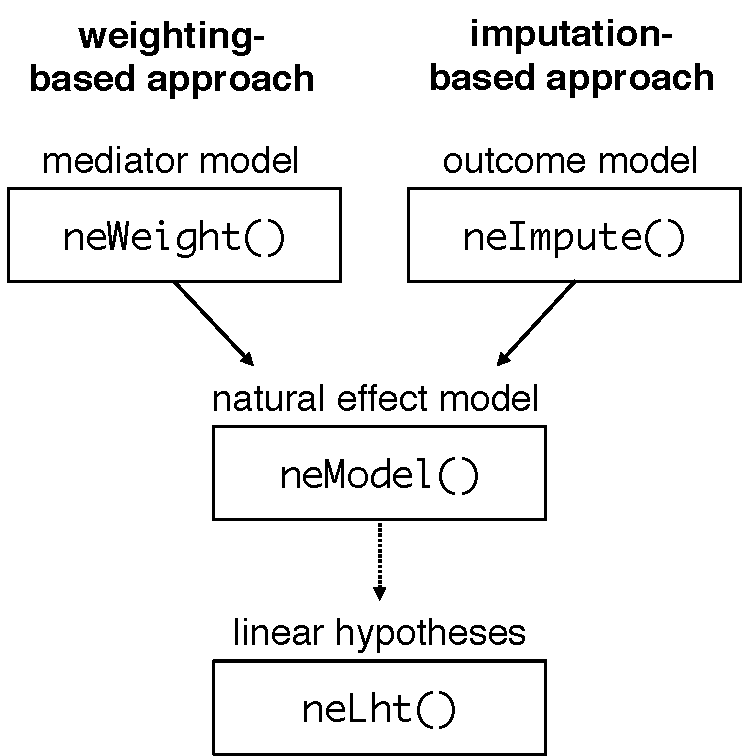
\includegraphics[width=6cm]{workflow.pdf}
  \caption{Workflow of the \pkg{medflex} package.}
  \label{fig:workflow}
\end{figure}
\subsection{Weighting-based approach}
One way to account for missingness in the expanded data is to standardize observed outcomes to the mediator distribution of the hypothetical exposure level $x^*$. Building on \citeauthor{Hong2010}'s \citeyearpar{Hong2010} ratio-of-mediator-probability weighting (RMPW) method, \cite{Lange2012} proposed to weight each observation in the expanded dataset by $$w_i = \dfrac{p_i(x^*)}{p_i(x)} = \dfrac{\Pr(M = M_i \vert X = x^*, C = C_i)}{\Pr(M = M_i \vert X = x, C = C_i)}.$$
\par For instance, for a binary exposure, $\E\{Y(0,M(0))|C\}$ and $\E\{Y(1,M(1))|C\}$ can readily be estimated from the observed data (under assumption~\ref{A1}) without weighting (i.e., as $x$ = $x^*$ the corresponding weights equal 1). To enable estimation of $\E\{Y(1,M(0))|C\}$ and $\E\{Y(0,M(1))|C\}$ RMPW aims to construct a `parallel' pseudo-population for each exposure group $x$ (within each stratum of $C$) with mediator values that would have been observed if each subject had been a member of the opposite exposure group $x^* = 1-x$. This is done by up-weighting individuals whose observed mediator value is more typical for the opposite exposure group than the exposure group to which they originally belong. Similarly, individuals whose observed mediator value is relatively more typical for the original exposure group are down-weighted.\footnote{\cite{Hong2015} gives a more detailed example which may provide more intuition into RMPW. Other weighting methods based on inverse odds (ratio) weighting \citep{Huber2013, TchetgenTchetgen2013} have been proposed recently. In contrast to RMPW these weighting methods rely on models for the exposure distribution (conditional on mediator and baseline covariates). Although these could easily be adopted within the natural effect model framework, these are currently not implemented in the \pkg{medflex} package.} 
\par Data expansion hence only requires $x^*$ to take on values different from the observed exposure to enable estimation of natural direct and indirect effects via the weighting-based approach, as illustrated in~Table~\ref{tab-exp2}. Estimates can then be obtained by regressing the observed outcome on $x$, $x^*$ and baseline covariates $C$, weighting each observation in the expanded dataset by its corresponding ratio-of-mediator-probability weight. This procedure easily extends to continuous exposures (see Section~\ref{contexp}) and/or mediators (provided probabilities are replaced by densities). The interested reader is referred to Appendix~\ref{app:weightest}, where a more technical account is given on the link between the weighting-based approach and the mediation formula.
\begin{table}[h]
\centering
\begin{tabular}{ccccccl}
\cmidrule[\heavyrulewidth](){1-5}
$i$& $X_i$ & $x$ & $x^*$ & $Y_i(x,M_i(x^*))$ & & $w_i$\\
\cmidrule(){1-5}
1 & 1 & 1 & 1 & $Y_1$ & & 1 \\
\rowcolor[gray]{.9}
1 & 1 & 1 & \textcolor{red}{\bf 0} & \textcolor{red}{$Y_1$} & \cellcolor{white} & \cellcolor{white}$\hat p_1(\textcolor{red}{\bf 0})/\hat p_1(1)$\\
2 & 0 & 0 & 0 & $Y_2$ & & 1\\
\rowcolor[gray]{.9}
2 & 0 & 0 & \textcolor{red}{\bf 1} & \textcolor{red}{$Y_2$} & \cellcolor{white} & \cellcolor{white}$\hat p_2(\textcolor{red}{\bf 1})/\hat p_2(0)$\\
\vdots & \vdots & \vdots & \vdots & \vdots & & \vdots \\
\cmidrule[\heavyrulewidth](){1-5}
\end{tabular}
\caption{Schematic display of the weighting-based approach.}\label{tab-exp2}
\end{table}

\subsubsection[]{Expanding the data and computing weights for the natural effect model}
Using the \pkg{medflex} package, expanding the dataset and calculating weights can be done in a single run, using the \code{neWeight} function. 
To calculate the weights, a model for the mediator needs to be fitted. For instance, in \proglang{R}, the simple linear model
\begin{align*}
\E(M|X,C) = \alpha_0 + \alpha_1 X + \alpha_2 C,
\end{align*}
can be fitted using the \code{glm} function:
\begin{Schunk}
\begin{Sinput}
R> medFit <- glm(negaff ~ factor(attbin) + gender + educ + age, 
+    family = gaussian, data = UPBdata)
\end{Sinput}
\end{Schunk}
Next, this fitted object needs to be specified as the first argument in \code{neWeight}, which in turn codes the first predictor variable in the \code{formula} argument as the exposure and then expands the data along hypothetical values of this variable. It is important to note here that, for successful data expansion, categorical exposures should be explicitly coded as factors in the \code{formula} if they are not yet coded as such in the dataset.
\begin{Schunk}
\begin{Sinput}
R> expData <- neWeight(medFit)
\end{Sinput}
\end{Schunk}
Inspecting the first rows of the resulting expanded dataset shows that for each individual two replications have been created:
\begin{Schunk}
\begin{Sinput}
R> head(expData, 4)
\end{Sinput}
\begin{Soutput}
  id attbin0 attbin1    att attcat negaff initiator gender educ age UPB
1  1       1       1  1.001      M   0.84    myself      F    M  41   1
2  1       1       0  1.001      M   0.84    myself      F    M  41   1
3  2       0       0 -0.709      L  -1.26      both      M    M  42   0
4  2       0       1 -0.709      L  -1.26      both      M    M  42   0
\end{Soutput}
\end{Schunk}
The new variables \code{attbin0} and \code{attbin1} correspond to hypothetical exposure values $x$ and $x^*$, respectively. By convention, the index `0' is used for parameters (and corresponding auxiliary variables) indexing natural direct effects, whereas the index `1' is used for parameters indexing natural indirect effects in the natural effect model.
\par To shorten code, one can instead choose to directly specify the \code{formula}, \code{family} and \code{data} arguments in \code{neWeight}.
\begin{Schunk}
\begin{Sinput}
R> expData <- neWeight(negaff ~ factor(attbin) + gender + educ + age,
+    data = UPBdata)
\end{Sinput}
\end{Schunk}
\par By default, \code{glm} is used as internal model-fitting function. However, other model-fitting functions can be specified in the \code{FUN} argument \citep[e.g., \code{vglm} from the \pkg{VGAM} package;][]{R:VGAM}.\footnote{In the current version of the package also \code{vglm} and \code{vgam} from the \pkg{VGAM} package and \code{gam} from the \pkg{gam} package \citep{R:gam} are supported. When specifying model-fitting functions other than \code{glm} in the \code{FUN} argument, one might need to specify the \code{family} argument differently. That is, in a way that is consistent with argument specification of that specific model-fitting function.}
\par Finally, the weights are stored as an attribute of the expanded dataset and can easily be retrieved using the generic \code{weights} function, e.g., for further inspection of their empirical distribution:
\begin{Schunk}
\begin{Sinput}
R> w <- weights(expData)
R> head(w, 10)
\end{Sinput}
\begin{Soutput}
 [1] 1.000 0.640 1.000 0.494 1.000 0.475 1.000 1.211 1.000 0.326
\end{Soutput}
\end{Schunk}

\subsubsection[]{Fitting the natural effect model on the expanded data}
After expanding the data and calculating regression weights for each of the replicates, the natural effect model can be fitted using the \code{neModel} function. Argument specification for this function is similar to that of the \code{glm} function, which is called internally. However, the \code{formula} argument now must be specified in function of the variables from the expanded dataset. The latter, in turn, needs to be specified via the \code{expData} argument. \code{neModel} automatically extracts the regression weights from this expanded dataset and applies them for model fitting.
\par Default \code{glm} standard errors tend to be downwardly biased as the uncertainty inherent to prediction of the weights based on the estimated mediator model is not taken into account. For this reason, \code{neModel} returns bootstrapped standard errors. In order to approximate the sampling distribution of each of the natural effect model parameters, the applied non-parametric bootstrap procedure repeatedly resamples the original data with replacement. For each replication, all aforementioned steps are repeated and estimates of the natural effect model parameters are obtained. The resulting bootstrap distribution can then be used for statistical inference. By refitting the same model for the mediator distribution to each bootstrap sample and recalculating ratio-of-mediator-probability weights for the (subsequently) expanded bootstrap samples, uncertainty related to estimation of the mediator model is incorporated into the bootstrapped standard errors. The number of bootstrap replications defaults to 1000 and can be set in the \code{nBoot} argument:
\begin{Schunk}
\begin{Sinput}
R> neMod1 <- neModel(UPB ~ attbin0 + attbin1 + gender + educ + age,
+    family = binomial("logit"), expData = expData)
\end{Sinput}
\end{Schunk}
The \code{summary} table of the resulting natural effect model object provides these bootstrap standard errors along with corresponding Wald-type $z$~statistics and $p$~values.
\begin{Schunk}
\begin{Sinput}
R> summary(neMod1)
\end{Sinput}
\begin{Soutput}
Natural effect model
with standard errors based on the non-parametric bootstrap
---
Exposure: attbin 
Mediator(s): negaff 
---
Parameter estimates:
             Estimate Std. Error z value Pr(>|z|)    
(Intercept) -0.925206   0.955118  -0.969 0.332704    
attbin01     0.395924   0.224899   1.760 0.078331 .  
attbin11     0.351969   0.091480   3.847 0.000119 ***
genderM      0.275968   0.247549   1.115 0.264936    
educM        0.167009   0.768958   0.217 0.828061    
educH        0.423350   0.780908   0.542 0.587732    
age         -0.009449   0.013178  -0.717 0.473354     
---
Signif. codes:  0 ‘***’ 0.001 ‘**’ 0.01 ‘*’ 0.05 ‘.’ 0.1 ‘ ’ 1
\end{Soutput}
\end{Schunk}
\par As an alternative, robust standard errors based on the sandwich estimator \citep{Liang1986} can be requested by setting \code{se = "robust"}. Calculation of these standard errors is less computer-intensive and is available for natural effect models with working models fitted via the \code{glm} function.
\begin{Schunk}
\begin{Sinput}
R> neMod1 <- neModel(UPB ~ attbin0 + attbin1 + gender + educ + age,
+    family = binomial("logit"), expData = expData, se = "robust")
R> summary(neMod1)
\end{Sinput}
\begin{Soutput}
Natural effect model
with robust standard errors based on the sandwich estimator
---
Exposure: attbin 
Mediator(s): negaff 
---
Parameter estimates:
            Estimate Std. Error z value Pr(>|z|)    
(Intercept) -0.92521    0.71463   -1.29    0.195    
attbin01     0.39592    0.21761    1.82    0.069 .  
attbin11     0.35197    0.08939    3.94  8.2e-05 ***
genderM      0.27597    0.23370    1.18    0.238    
educM        0.16701    0.50065    0.33    0.739    
educH        0.42335    0.50917    0.83    0.406    
age         -0.00945    0.01227   -0.77    0.441    
---
Signif. codes:  0 '***' 0.001 '**' 0.01 '*' 0.05 '.' 0.1 ' ' 1
\end{Soutput}
\end{Schunk}

\subsubsection{Interpreting model parameters}
Exponentiating the model parameter estimates provides estimates that can be interpreted as odds ratios. For instance, for a subject with baseline covariate levels $C$, altering the level of anxious attachment from low (=0) to high (=1), while controlling negative affectivity at levels as naturally observed at any given level of anxious attachment $x$, increases the odds of displaying unwanted pursuit behaviors with a factor
\begin{align*}
\widehat{\mbox{OR}}^{\text{NDE}}_{1,0|C} &= \frac{\mbox{odds}\left\{Y(1,M(x))=1|C\right\}}{\mbox{odds}\left\{Y(0,M(x))=1|C\right\}} = \exp(\hat{\beta_1}) = \exp(0.3959) = 1.49.
\end{align*}
Altering levels of negative affectivity as observed at low anxious attachment scores to levels that would have been observed at high anxious attachment scores, while controlling their anxious attachment score at any given level $x$, increases the odds of displaying unwanted pursuit behaviors with a factor
\begin{align*}
\widehat{\mbox{OR}}^{\text{NIE}}_{1,0|C} &= \frac{\mbox{odds}\left\{Y(x,M(1))=1|C\right\}}{\mbox{odds}\left\{Y(x,M(0))=1|C\right\}} = \exp(\hat{\beta_2}) = \exp(0.352) = 1.42.
\end{align*}
Wald-type confidence intervals can be obtained by applying the \code{confint} function to the natural effect model object. The confidence level defaults to 95\%, but can be changed via the \code{level} argument. By exponentiating the intervals on the logit scale, we can obtain the corresponding 95\% confidence intervals (based on the robust standard errors) on the odds ratio scale:
\begin{Schunk}
\begin{Sinput}
R> exp(confint(neMod1)[c("attbin01", "attbin11"), ])
\end{Sinput}
\begin{Soutput}
         95% LCL 95% UCL
attbin01    0.97    2.28
attbin11    1.19    1.69
\end{Soutput}
\end{Schunk}
If standard errors are obtained via the bootstrap procedure, bootstrap confidence intervals are returned. The default type is calculated based on a first order normal approximation (\code{type = "norm"}), but other types of bootstrap confidence intervals (such as basic bootstrap, bootstrap percentile and bias-corrected and accelerated confidence intervals) can be obtained by setting the \code{type} argument to the desired type.\footnote{The \code{type} argument in \code{confint} corresponds to that of the \code{boot.ci} function from the \pkg{boot} package \citep{R:boot}, which is called internally.}

\newpage
\subsection{Imputation-based approach}\label{imp-appr}
The second approach avoids reliance on a model for the mediator distribution and instead requires fitting a working model for the outcome mean \citep{Vansteelandt2012}. By setting $x^*$ (rather than $x$) equal to the observed exposure $X$, unobserved nested counterfactuals can be imputed using any appropriate model for the outcome mean. That is, since the potential intermediate outcome $M(x^*)$ equals the observed mediator $M$ within the subgroup with exposure $X = x^*$, $Y(x,M(x^*))$ equals $Y(x,M)$ for all individuals in that exposure group. The latter can then be imputed using fitted values $\hat \E(Y \vert X = x,M,C)$ based on an appropriate model for the outcome mean, henceforth referred to as the imputation model, with exposure $X$ set to $x$ and with mediator $M$ and baseline covariates $C$ set to their observed values. This approach easily accommodates missing outcomes in the original dataset, as the corresponding nested counterfactuals can likewise be imputed.
\par In contrast to the weighting-based approach, data expansion only requires $x$ to take on values different from the observed exposure to enable estimation of natural direct and indirect effects, as illustrated in~Table~\ref{tab-exp3}. Estimates can finally be obtained upon fitting a natural effect model to the imputed dataset. For ease of implementation, observed nested counterfactuals are imputed as well in the \pkg{medflex} package.\footnote{Simulation studies (not shown here) have shown that this procedure does not lead to bias or loss of efficiency.} In Appendix~\ref{app:impest}, we demonstrate the link between the mediation formula and the imputation-based approach by showing how the former can be rewritten as an expression that prescribes estimating nested counterfactuals by calculating the mean of imputed nested counterfactuals, conditional on $x$, $x^*$ and $C$.
\begin{table}[h]
\centering
\begin{tabular}{ccccc}
\toprule
$i$ & $X_i$ & $x$ & $x^*$ & $Y_i(x,M_i(x^*))$\\
\midrule
1 & 1 & 1 & 1 & $Y_1$\\
\rowcolor[gray]{.9}
1 & 1 & \textcolor{red}{\bf 0} & 1 & \textcolor{red}{$\hat Y_1({\bf 0},M_1)$}\\ 
2 & 0 & 0 & 0 & $Y_2$\\
\rowcolor[gray]{.9}
2 & 0 & \textcolor{red}{\bf 1} & 0 & \textcolor{red}{$\hat Y_2({\bf 1},M_2)$}\\ 
\vdots & \vdots & \vdots & \vdots & \vdots\\
\bottomrule
\end{tabular}
\caption{Schematic display of the imputation-based approach. $\hat Y_i(x,M_i)$ represent the imputed counterfactual outcomes.}\label{tab-exp3}
\end{table}

\subsubsection[]{Expanding the data and imputing nested counterfactuals}\label{subsec:expimp}
Although application of the imputation-based approach is similar to that of the weighting-based approach, it differs in some key respects. These differences are mainly captured by differences between the functions \code{neWeight} and \code{neImpute}. Argument specification of this function is identical to that of \code{neWeight}, unless indicated otherwise.
\par As for the weighted-based approach, the first step amounts to fitting a working model. Instead of a model for the mediator, the imputation-based approach requires fitting a mean model for the outcome. Moreover, this model should at least reflect the structure of natural effect model~\eqref{eq:nemodelnoia} (i.e., it should at least contain all terms of the natural effect model with $x^*$ replaced by $M$). For instance, a simple logistic regression model
\begin{align*}
\mbox{logit} \Pr(Y=1|X,M,C) = \gamma_0 + \gamma_1 X + \gamma_2 M + \gamma_3 C,
\end{align*}
can be fitted in \proglang{R} using the \code{glm} function:
\begin{Schunk}
\begin{Sinput}
R> impFit <- glm(UPB ~ factor(attbin) + negaff + gender + educ + age,
+    family = binomial("logit"), data = UPBdata)
\end{Sinput}
\end{Schunk}
In order for \code{neImpute} to identify the predictor variables in the \code{formula} argument correctly as either exposure, mediator(s) or baseline covariates, they need to be entered in a particular order. That is, the first predictor variable again needs to point to the exposure and the second to the mediator. All other predictors are automatically coded as baseline covariates. It is important to adhere to this prespecified order to enable \code{neImpute} to create valid pointers to these different types of predictor variables. This requirement extends to the use of operators different from the \code{+} operator, such as the \code{:} and \code{*} operators (when e.g., adding interaction terms). For instance, the formula expressions \code{Y ~ X + M + C1 + C2 + X:C1 + M:C1}, \code{Y ~ X + M + X:C1 + M:C1 + C1 + C2}, \code{Y ~ (X + M) * C1 + C2} and \code{Y ~ X * C1 + M * C1 + C2} all impose the same structural form for the imputation model. However, only for the former three expressions, correct pointers to exposure, mediator and baseline covariates will be created, as the order of occurence of each of the unique predictor variables is identical in all three specifications, but not in the latter.
\par This fitted object then needs to be entered as the first argument in \code{neImpute}:
\begin{Schunk}
\begin{Sinput}
R> expData <- neImpute(impFit)
\end{Sinput}
\end{Schunk}
Alternatively, the \code{formula}, \code{family} and \code{data} arguments can be directly specified in \code{neImpute}:
\begin{Schunk}
\begin{Sinput}
R> expData <- neImpute(UPB ~ factor(attbin) + negaff + gender + educ + age,
+    family = binomial("logit"), data = UPBdata)
\end{Sinput}
\end{Schunk}
Similar to \code{neWeight}, \code{neImpute} first expands the data along hypothetical exposure values. Instead of calculating weights for these new observations, \code{neImpute} then imputes the nested counterfactual outcomes by fitted values based on the imputation model. As illustrated below, the resulting expanded dataset includes two imputed nested counterfactual outcomes for each subject. The outcomes are no longer binary, but are substituted by conditional mean imputations.
\begin{Schunk}
\begin{Sinput}
R> head(expData, 4)
\end{Sinput}
\begin{Soutput}
  id attbin0 attbin1    att attcat negaff initiator gender educ age   UPB
1  1       1       1  1.001      M   0.84    myself      F    M  41 0.492
2  1       0       1  1.001      M   0.84    myself      F    M  41 0.384
3  2       0       0 -0.709      L  -1.26      both      M    M  42 0.187
4  2       1       0 -0.709      L  -1.26      both      M    M  42 0.263
\end{Soutput}
\end{Schunk}

\subsubsection[]{Fitting the natural effect model on the imputed data}
After expanding and imputing the data, specifying the natural effect model can be done as for the weighting-based approach:
\begin{Schunk}
\begin{Sinput}
R> neMod1 <- neModel(UPB ~ attbin0 + attbin1 + gender + educ + age,
+    family = binomial("logit"), expData = expData, se = "robust")
\end{Sinput}
\end{Schunk}
Again, bootstrap or robust standard errors are reported in the output of the \code{summary} function, in order to account for the uncertainty inherent to the working model (i.e., in this case, the imputation model):
\begin{Schunk}
\begin{Sinput}
R> summary(neMod1)
\end{Sinput}
\begin{Soutput}
Natural effect model
with robust standard errors based on the sandwich estimator
---
Exposure: attbin 
Mediator(s): negaff 
---
Parameter estimates:
            Estimate Std. Error z value Pr(>|z|)    
(Intercept)  -0.9216     0.6892   -1.34     0.18    
attbin01      0.4015     0.2134    1.88     0.06 .  
attbin11      0.3407     0.0805    4.23  2.3e-05 ***
genderM       0.2940     0.2250    1.31     0.19    
educM         0.3462     0.4817    0.72     0.47    
educH         0.5143     0.4878    1.05     0.29    
age          -0.0122     0.0119   -1.02     0.31    
---
Signif. codes:  0 '***' 0.001 '**' 0.01 '*' 0.05 '.' 0.1 ' ' 1
\end{Soutput}
\end{Schunk}
Natural direct and indirect effect odds ratio estimates and their confidence intervals can be obtained as before. 

\section{Dealing with different types of variables}\label{types}
In the previous section, we used a dichotomized version of the continuous exposure variable \code{att}. However, the natural effect model framework easily extends to different types of exposure, mediator or outcome variables. In the following two sections, we give a detailed description on how to fit natural effect models with multicategorical (i.e., ordinal or nominal) and continuous exposures. In these sections, as well as throughout the remainder of this paper, we will focus on the imputation-based approach when introducing new features of the \pkg{medflex} package. Unless indicated otherwise, the weighting-based approach can be applied analogously.
\par An overview of the types of mediators and outcomes the \pkg{medflex} package can currently handle, is given in Table~\ref{tab-vartypes}. When using the weighting-based approach, models for binary, count and continuous mediators can be fitted using the \code{glm} function or the \code{vglm} function from the \pkg{VGAM} package. Models for nominal mediators, on the other hand, can only be fitted using the \code{vglm} function (setting \code{family = multinomial}).\footnote{In the current version of the package, when using working models for weighting (either when adopting the weighting-based approach or when fitting population-average natural effect models), robust standard errors are only available if these working models are fitted using \code{glm} and their outcomes (i.e., either an exposure or a mediator) follow either a normal, binomial or Poisson distribution.} Although models for ordinal mediators are not compatible with the \code{neWeight} function, ordered factors can easily be treated as nominal variables. Finally, the imputation-based approach can deal with virtually any type of mediator as it does not require the specification of a mediator model.
\begin{table}[t]
\centering
\begin{tabular}{lcccccc}
\toprule
& \multicolumn{6}{c}{\textit{Outcome type}}\\
\cmidrule{2-7}
 & \multicolumn{2}{c}{Binary} & \multicolumn{2}{c}{Count} & \multicolumn{2}{c}{Continuous}\\
\cmidrule{2-7}
\textit{Mediator type} & \code{neWeight} & \code{neImpute} & \code{neWeight} & \code{neImpute} & \code{neWeight} & \code{neImpute} \\
\midrule
Binary & \ding{51} & \ding{51} & \ding{51} & \ding{51} & \ding{51} & \ding{51}\\
Count & \ding{51} & \ding{51} & \ding{51} & \ding{51} & \ding{51} & \ding{51}\\
Continuous & \ding{51} & \ding{51} & \ding{51} & \ding{51} & \ding{51} & \ding{51}\\
Ordinal &  & \ding{51} &  & \ding{51} &  & \ding{51}\\
Nominal & \ding{51}$^*$ & \ding{51} & \ding{51}$^*$ & \ding{51} & \ding{51}$^*$ & \ding{51}\\
\bottomrule
\end{tabular}
\caption{Types of variables that can be dealt with in the \pkg{medflex} package. Natural effect models are currently restricted to models that can be fitted with the \code{glm} function. `*' indicates that robust standard errors are not available.
}\label{tab-vartypes}
\end{table}

\subsection{Multicategorical exposures}
Methods for dealing with multicategorical treatments or exposures, as encountered in e.g., multiple intervention studies, in which multiple experimental conditions are compared to a control condition, have rarely been described within the mediation literature \citep[although see][for some notable exceptions]{Hayes2014,R:mediation}.
\par In this section, we illustrate how to expand the dataset and fit natural effect models when using a multicategorical exposure. In this example, instead of using the binary exposure variable \code{attbin}, we use a discretized version of anxious attachment style, named \code{attcat} (with \code{L} indicating low, \code{M} indicating intermediate and \code{H} indicating high anxious attachment levels). 
\par Inspecting the first rows of the expanded dataset shows that the number of replications for each subject again corresponds to the number of unique levels of the categorical exposure variable. That is, the auxiliary variable $x^*$ (\code{attcat1}) is fixed to the observed exposure, whereas the other, $x$ (\code{attcat0}), enumerates all potential exposure levels.
\begin{Schunk}
\begin{Sinput}
R> expData <- neImpute(UPB ~ attcat + negaff + gender + educ + age,
+    family = binomial("logit"), data = UPBdata)
R> head(expData)
\end{Sinput}
\begin{Soutput}
  id attcat0 attcat1    att attbin negaff initiator gender educ age   UPB
1  1       M       M  1.001      1   0.84    myself      F    M  41 0.468
2  1       H       M  1.001      1   0.84    myself      F    M  41 0.558
3  1       L       M  1.001      1   0.84    myself      F    M  41 0.366
4  2       L       L -0.709      0  -1.26      both      M    M  42 0.182
5  2       M       L -0.709      0  -1.26      both      M    M  42 0.253
6  2       H       L -0.709      0  -1.26      both      M    M  42 0.327
\end{Soutput}
\end{Schunk}
The \code{summary} table returns estimates for the natural direct and indirect effect log odds ratios comparing intermediate and high anxious attachment levels to low levels of anxious attachment (i.e., the reference level).
\begin{Schunk}
\begin{Sinput}
R> neMod <- neModel(UPB ~ attcat0 + attcat1 + gender + educ + age,
+    family = binomial("logit"), expData = expData, se = "robust")
R> summary(neMod)
\end{Sinput}
\begin{Soutput}
Natural effect model
with robust standard errors based on the sandwich estimator
---
Exposure: attcat 
Mediator(s): negaff 
---
Parameter estimates:
            Estimate Std. Error z value Pr(>|z|)    
(Intercept)  -0.9616     0.6976   -1.38  0.16807    
attcat0M      0.3921     0.2365    1.66  0.09729 .  
attcat0H      0.7239     0.3105    2.33  0.01975 *  
attcat1M      0.3012     0.0797    3.78  0.00016 ***
attcat1H      0.5218     0.1314    3.97  7.2e-05 ***
genderM       0.2700     0.2266    1.19  0.23336    
educM         0.3279     0.4817    0.68  0.49601    
educH         0.4826     0.4877    0.99  0.32239    
age          -0.0127     0.0121   -1.05  0.29510    
---
Signif. codes:  0 '***' 0.001 '**' 0.01 '*' 0.05 '.' 0.1 ' ' 1
\end{Soutput}
\end{Schunk}
Overall assessment of natural effects (i.e., a joint comparison of all levels of the exposure) cannot be based on the default \code{summary} output, but instead requires an Anova table for the natural effect model, which can be obtained using the \code{Anova} function from the \pkg{car} package \citep{R:car}:
\begin{Schunk}
\begin{Sinput}
R> library("car")
R> Anova(neMod)
\end{Sinput}
\begin{Soutput}
Analysis of Deviance Table (Type II tests)

Response: UPB
            Df Chisq Pr(>Chisq)    
attcat0      2  5.98       0.05 .  
attcat1      2 19.11    7.1e-05 ***
gender       1  1.42       0.23    
educ         2  1.17       0.56    
age          1  1.10       0.30    
Residuals 1146                     
---
Signif. codes:  0 '***' 0.001 '**' 0.01 '*' 0.05 '.' 0.1 ' ' 1
\end{Soutput}
\end{Schunk}
Both type-II (the default) and type-III Anova tables can be requested by specifying the desired type via the \code{type} argument. This table includes corresponding Wald $\chi^2$ tests for multivariate hypotheses which account for the uncertainty inherent to the working model. The output suggests that the natural direct and indirect effect odds differ significantly between the three exposure levels. 

\subsection{Continuous exposures}\label{contexp}
In contrast to the \pkg{mediation} package, hypothesis testing for natural direct and indirect effects along the entire support of continuous exposures is facilitated by defining causal effects on their most natural scale. In this section, we use the continuous variable \code{att}, a standardized version of the original anxious attachment variable. 
\par For continuous variables, expanding the dataset along unobserved ($x$, $x^*$) combinations requires a slightly adapted approach than for categorical exposures. Instead of enumerating all exposure levels to construct auxiliary variables $x$ and $x^*$ for each subject, \cite{Vansteelandt2012} proposed to draw specific quantiles from the conditional density of the exposure given baseline covariates. By default, these hypothetical exposure levels are drawn from a linear model for the exposure, conditional on a linear combination of all covariates specified in the working model.\footnote{If one wishes to use another model for the exposure, this default model specification can be overruled by referring to a fitted model object in the \code{xFit} argument. Misspecification of this sampling model does not induce bias in the estimated coefficients and standard errors of the natural effect model.}
\par Both \code{neWeight} and \code{neImpute} allow to choose the number of draws to sample from this conditional density via the \code{nRep} argument (which defaults to 5).\footnote{We recommend to use a minimum of 3 draws. Although finite sample bias and sampling variability can be reduced to some extent by choosing a larger number of draws, simulations have shown this gain to be ignorable when choosing more than 5 draws \citep{Vansteelandt2012}.}
\begin{Schunk}
\begin{Sinput}
R> expData <- neImpute(UPB ~ att + negaff + gender + educ + age, 
+    family = binomial("logit"), data = UPBdata, nRep = 3)
R> head(expData)
\end{Sinput}
\begin{Soutput}
  id      att0   att1 attbin attcat negaff initiator gender educ age   UPB
1  1 -1.64e+00  1.001      1      M   0.84    myself      F    M  41 0.309
2  1  8.02e-06  1.001      1      M   0.84    myself      F    M  41 0.429
3  1  1.64e+00  1.001      1      M   0.84    myself      F    M  41 0.557
4  2 -1.66e+00 -0.709      0      L  -1.26      both      M    M  42 0.149
5  2 -1.82e-02 -0.709      0      L  -1.26      both      M    M  42 0.227
6  2  1.63e+00 -0.709      0      L  -1.26      both      M    M  42 0.330
\end{Soutput}
\end{Schunk}
Specification of the natural effect model via \code{neModel} can be done as described before:
\begin{Schunk}
\begin{Sinput}
R> neMod1 <- neModel(UPB ~ att0 + att1 + gender + educ + age,
+    family = binomial("logit"), expData = expData, se = "robust")
R> summary(neMod1)
\end{Sinput}
\begin{Soutput}
Natural effect model
with robust standard errors based on the sandwich estimator
---
Exposure: att 
Mediator(s): negaff 
---
Parameter estimates:
            Estimate Std. Error z value Pr(>|z|)    
(Intercept)  -0.4873     0.6862   -0.71   0.4776    
att0          0.2923     0.1091    2.68   0.0074 ** 
att1          0.2018     0.0470    4.29  1.8e-05 ***
genderM       0.2671     0.2274    1.17   0.2402    
educM         0.2679     0.4894    0.55   0.5841    
educH         0.4103     0.4959    0.83   0.4080    
age          -0.0120     0.0122   -0.99   0.3236    
---
Signif. codes:  0 '***' 0.001 '**' 0.01 '*' 0.05 '.' 0.1 ' ' 1
\end{Soutput}
\end{Schunk}
\par The output illustrates that defining natural effects on the (log) odds ratio scale allows to capture each of these effects along the entire support of the exposure by a single parameter. For instance, for a subject with baseline covariate levels $C$, the direct and indirect effects of one standard deviation increase in anxious attachment level (i.e., from $x$ to $x+1$) correspond to an increase in the odds of displaying unwanted pursuit behaviors by a factor 
\begin{align*}
\widehat{\mbox{OR}}^{\text{NDE}}_{x+1,x|C} &= \frac{\mbox{odds}\left\{Y(x+1,M(x))=1|C\right\}}{\mbox{odds}\left\{Y(x,M(x))=1|C\right\}} = \exp(\hat{\beta_1}) = \exp(0.29) = 1.34,
\end{align*}
and 
\begin{align*}
\widehat{\mbox{OR}}^{\text{NIE}}_{x+1,x|C} &= \frac{\mbox{odds}\left\{Y(x,M(x+1))=1|C\right\}}{\mbox{odds}\left\{Y(x,M(x))=1|C\right\}} = \exp(\hat{\beta_2}) = \exp(0.2) = 1.22,
\end{align*}
respectively, regardless of the initial level $x$. Defining natural effects on the risk difference scale (as in the \pkg{mediation} package) would not have enabled to capture these by a single parameter along the entire support of the exposure, because of induced non-additivity \citep[an artificial example illustrating this induced non-additivity is given in Figure 4 of][]{Loeys2013a}.
\par Throughout the remainder of the paper, we will continue to use the original continuous exposure variable, \code{att}.

\newpage
\section{Effect modification of natural effects}\label{modmed}
\subsection{Exposure-mediator interactions}\label{subsec:ia}
So far, the considered natural effect models reflected the assumption that exposure and mediator do not interact in their effect on the outcome (on the scale defined by the link function). In particular, the natural direct effect odds ratio 
\begin{align*}
\mbox{OR}^{\text{NDE}}_{1,0|C}(x^*) = \frac{\mbox{odds}\left\{Y(1,M(x^*))=1|C\right\}}{\mbox{odds}\left\{Y(0,M(x^*))=1|C\right\}}
\end{align*}
was postulated to be the same for each choice of mediator level $M(x^*)$, and hence for each choice of reference exposure level $x^*$, at which the mediator is evaluated. Similarly, the natural indirect effect odds ratio 
\begin{align*}
\mbox{OR}^{\text{NIE}}_{1,0|C}(x) = \frac{\mbox{odds}\left\{Y(x,M(1))=1|C\right\}}{\mbox{odds}\left\{Y(x,M(0))=1|C\right\}}
\end{align*}
was postulated to be constant across different choices of $x$ at which the outcome is evaluated. 
In other words, the effects \cite{Greenland1992} referred to as the \emph{pure} direct effect, $\mbox{OR}^{\text{NDE}}_{1,0|C}(0)$, and \emph{total} direct effect, $\mbox{OR}^{\text{NDE}}_{1,0|C}(1)$, were assumed to be equal. Likewise, the \emph{pure} indirect effect, $\mbox{OR}^{\text{NIE}}_{1,0|C}(0)$, and \emph{total} indirect effect, $\mbox{OR}^{\text{NIE}}_{1,0|C}(1)$, were assumed to be equal. However, in many studies, these assumptions may not be plausible.
\par As pointed out by \cite{VanderWeele2013a}, total causal effects can be decomposed into a pure direct effect, a pure indirect effect and a mediated interactive effect. On an additive scale, the latter can be described as either the difference between total direct and pure direct effects or as the difference between total indirect and pure indirect effects. Similarly, the total effect odds ratio 
\begin{align*}
\mbox{OR}_{1,0|C} = \frac{\mbox{odds}\left\{Y(1,M(1))=1|C\right\}}{\mbox{odds}\left\{Y(0,M(0))=1|C\right\}}
\end{align*}
can be expressed as the product $$\mbox{OR}^{\text{NDE}}_{1,0|C}(0) \times \mbox{OR}^{\text{NIE}}_{1,0|C}(0) \times \dfrac{\mbox{OR}^{\text{NDE}}_{1,0|C}(1)}{\mbox{OR}^{\text{NDE}}_{1,0|C}(0)} = \mbox{OR}^{\text{NDE}}_{1,0|C}(0) \times \mbox{OR}^{\text{NIE}}_{1,0|C}(0) \times \dfrac{\mbox{OR}^{\text{NIE}}_{1,0|C}(1)}{\mbox{OR}^{\text{NIE}}_{1,0|C}(0)}$$
of the pure direct and pure indirect effect odds ratios and the mediated interaction odds ratio.
Rather than reflecting the \emph{difference} between total and pure direct or indirect effects, the mediated interaction odds ratio corresponds to the \emph{ratio} of total and pure direct or indirect effect odds ratios.
\par In a logistic natural effect model, testing for exposure-mediator interaction amounts to testing whether the mediated interaction odds ratio differs from 1, or equivalently, on the scale of the linear predictor, whether the corresponding log odds ratio, $\beta_3^\prime$ in natural effect model
\begin{align}\label{eq:nemodelia}
\mbox{logit} \Pr\left\{Y(x,M(x^*))=1|C\right\} = \beta_0^\prime + \beta_1^\prime x + \beta_2^\prime x^* + \beta_3^\prime xx^* + \beta_4^\prime C,
\end{align}
differs from 0. When including this interaction term in the outcome model, $\beta_1^\prime$ and $\beta_2^\prime$ encode the pure direct and indirect effect log odds ratios, respectively.
\par When applying the imputation-based approach, the working model needs to at least reflect the structure of the final natural effect model (as has been pointed out in Section~\ref{imp-appr}). This requires the user to first (re)fit the imputation model accordingly. For instance, a minimal imputation model for natural effect model~\eqref{eq:nemodelia} would be the logistic regression model
\begin{align*}
\mbox{logit} \Pr(Y=1|X,M,C) = \gamma_0^\prime + \gamma_1^\prime X + \gamma_2^\prime M + \gamma_3^\prime XM + \gamma_4^\prime C.
\end{align*}
The output of the corresponding natural effect model object suggests there is no evidence for mediated interaction at the 5\% significance level ($p = .0541$).
\begin{Schunk}
\begin{Sinput}
R> expData <- neImpute(UPB ~ att * negaff + gender + educ + age,
+    family = binomial("logit"), data = UPBdata)
R> neMod2 <- neModel(UPB ~ att0 * att1 + gender + educ + age,
+    family = binomial("logit"), expData = expData, se = "robust")
R> summary(neMod2)
\end{Sinput}
\begin{Soutput}
Natural effect model
with robust standard errors based on the sandwich estimator
---
Exposure: att 
Mediator(s): negaff 
---
Parameter estimates:
            Estimate Std. Error z value Pr(>|z|)    
(Intercept)  -0.3949     0.6800   -0.58   0.5614    
att0          0.2950     0.1102    2.68   0.0074 ** 
att1          0.1817     0.0467    3.90  9.8e-05 ***
genderM       0.2815     0.2263    1.24   0.2135    
educM         0.1798     0.4857    0.37   0.7113    
educH         0.3105     0.4929    0.63   0.5287    
age          -0.0139     0.0122   -1.14   0.2545    
att0:att1     0.0698     0.0363    1.93   0.0541 .  
---
Signif. codes:  0 '***' 0.001 '**' 0.01 '*' 0.05 '.' 0.1 ' ' 1
\end{Soutput}
\end{Schunk}

\subsection{Effect modification by baseline covariates}
One might additionally wish to determine whether direct or indirect effects generalize across different strata of the population and across different conditions.
\par In our example, researchers might for instance investigate whether the extent to which the effect of anxious attachment level on engaging in UPBs is mediated through the experience of negative affectivity differs between men and women or between people with different education levels \citep{Muller2005, Preacher2007}. This moderated mediation hypothesis can be probed by allowing the conditional indirect effect, as indexed by $\beta_2$ in model~\eqref{eq:nemodelnoia}, to depend on gender, $C_1$, as expressed in model~\eqref{eq:nemodelmodmed1}:
\begin{align}\label{eq:nemodelmodmed1}
\mbox{logit} \Pr\left\{Y(x,M(x^*))=1|C\right\} = \beta_0^{\prime\prime} + \beta_1^{\prime\prime} x + \beta_2^{\prime\prime} x^* + \beta_3^{\prime\prime} x^* C_1 + \beta_4^{\prime\prime} C.
\end{align}
The amount of effect modification by gender in this model is then simply captured by $\beta^{\prime\prime}_3$.
\begin{Schunk}
\begin{Sinput}
R> impData <- neImpute(UPB ~ (att + negaff) * gender + educ + age,
+    family = binomial("logit"), data = UPBdata)
R> neMod3 <- neModel(UPB ~ att0 + att1 * gender + educ + age,
+    family = binomial("logit"), expData = impData, se = "robust")
R> summary(neMod3)
\end{Sinput}
\begin{Soutput}
Natural effect model
with robust standard errors based on the sandwich estimator
---
Exposure: att 
Mediator(s): negaff 
---
Parameter estimates:
             Estimate Std. Error z value Pr(>|z|)   
(Intercept)   -0.4731     0.6860   -0.69   0.4904   
att0           0.2850     0.1069    2.67   0.0077 **
att1           0.1441     0.0583    2.47   0.0134 * 
genderM        0.2591     0.2278    1.14   0.2553   
educM          0.2718     0.4903    0.55   0.5793   
educH          0.4166     0.4975    0.84   0.4024   
age           -0.0123     0.0122   -1.00   0.3153   
att1:genderM   0.1598     0.1016    1.57   0.1156   
---
Signif. codes:  0 '***' 0.001 '**' 0.01 '*' 0.05 '.' 0.1 ' ' 1
\end{Soutput}
\end{Schunk}
\par The output suggests that the natural indirect effect does not differ significantly between men and women ($p = 0.1156$).
\par In a similar way, researchers can gauge effect modification by education level. Suppose, for instance, that one wishes to test whether education level moderates both the direct and indirect effect. This can be done by fitting the natural effect model
\begin{align}\label{eq:nemodelmodmed2}
\mbox{logit} \Pr\left\{Y(x,M(x^*))=1|C\right\} &= \beta_0^{\star} + \beta_1^{\star} x + \beta_2^{\star} x^* + \beta_3^{\star} x C_{2,1} + \beta_4^{\star} x C_{2,2}\nonumber\\ & \phantom{= \beta_0^{\star} + \beta_1^{\star} x + \beta_2^{\star} x^*} + \beta_5^{\star} x^* C_{2,1} + \beta_6^{\star} x^* C_{2,2} + \beta_7^{\star} C,
\end{align}
with $C_{2,1}$ and $C_{2,2}$ dummy variables encoding the three education levels. Effect modification of the natural indirect (direct) effect by education level in model~\eqref{eq:nemodelmodmed2} is then captured by $\beta_5^{\star}$ and $\beta_6^{\star}$ ($\beta_3^{\star}$ and $\beta_4^{\star}$).
\begin{Schunk}
\begin{Sinput}
R> impData <- neImpute(UPB ~ (att + negaff) * educ + gender + age,
+    family = binomial("logit"), data = UPBdata)
R> neMod4 <- neModel(UPB ~ (att0 + att1) * educ + gender + age,
+    family = binomial("logit"), expData = impData, se = "robust")
\end{Sinput}
\end{Schunk}
Testing for moderation by a multicategorical variable calls for a multivariate test, which can again be obtained by requesting an Anova table for the natural effect model.

\newpage
\section{Tools for calculating and visualizing causal effect estimates}\label{tools}
In this section, we highlight tools that can aid in calculating and visualizing specific causal effect estimates of interest. These tools might prove useful for gaining insight, especially for more complex models including interaction terms involving natural effect parameters. 

\subsection{Linear combinations of parameter estimates}
Although effect estimates for e.g., the total causal effect can easily be obtained from the \code{summary} table of a natural effect model, its standard error and confidence interval cannot. To this end, the function \code{neLht}, which exploits the functionality of the \code{glht} function from the \pkg{multcomp} package \citep{R:multcomp} can be of use. This function enables the calculation of linear combinations of parameter estimates as well as their corresponding standard errors and confidence intervals based on the bootstrap or robust variance-covariance matrix of the natural effect model. 
\par For instance, in model~\eqref{eq:nemodelia}, the total direct and indirect effect can be expressed on the log odds scale as $\beta_1^\prime + \beta_3^\prime$ and $\beta_2^\prime + \beta_3^\prime$, respectively. Similarly, the total causal effect log odds ratio is captured by $\beta_1^\prime + \beta_2^\prime + \beta_3^\prime$. As the argument for the linear function, \code{linfct}, needs to be specified in terms of one or more linear hypotheses, these effects can be specified as illustrated below:
\begin{Schunk}
\begin{Sinput}
R> lht <- neLht(neMod2, linfct = c("att0 + att0:att1 = 0",
+    "att1 + att0:att1 = 0", "att0 + att1 + att0:att1 = 0"))
\end{Sinput}
\end{Schunk}
The corresponding odds ratios and their confidence intervals can be requested by exponentiating the coefficients and confidence intervals of the resulting object:
\begin{Schunk}
\begin{Sinput}
R> exp(cbind(coef(lht), confint(lht)))
\end{Sinput}
\begin{Soutput}
                             95% LCL 95% UCL
att0 + att0:att1        1.44    1.15    1.80
att1 + att0:att1        1.29    1.15    1.43
att0 + att1 + att0:att1 1.73    1.39    2.15
\end{Soutput}
\end{Schunk}
Separate univariate tests for linear hypothesis objects can be requested using the \code{summary} function:
\begin{Schunk}
\begin{Sinput}
R> summary(lht)
\end{Sinput}
\begin{Soutput}
Linear hypotheses for natural effect models
with standard errors based on the sandwich estimator
---
                        Estimate Std. Error z value Pr(>|z|)    
att0 + att0:att1          0.3648     0.1145    3.19   0.0014 ** 
att1 + att0:att1          0.2515     0.0553    4.55  5.4e-06 ***
att0 + att1 + att0:att1   0.5465     0.1118    4.89  1.0e-06 ***
---
Signif. codes:  0 '***' 0.001 '**' 0.01 '*' 0.05 '.' 0.1 ' ' 1
(Univariate p-values reported)
\end{Soutput}
\end{Schunk}
In contrast to the \code{summary} table for \code{glht} objects, which yields $p$~values that are adjusted for multiple testing, tests returned by the \code{summary} function applied to \code{neLht} objects report unadjusted univariate tests. Adjusted tests can be obtained by setting \code{test = adjusted()} \citep[for more details consult the help page of the \code{adjusted()} function from the \pkg{multcomp} package;][]{R:multcomp}.

\subsection{Effect decomposition}\label{effdecomp}
If interest is mainly focused on the natural effect parameters, the convenience function \code{neEffdecomp} can be used instead of \code{neLht}. This function automatically retains the natural effect estimates and generates a linear hypothesis object that reflects the most suitable effect decomposition:
\begin{Schunk}
\begin{Sinput}
R> effdecomp <- neEffdecomp(neMod2)
R> summary(effdecomp)
\end{Sinput}
\begin{Soutput}
Effect decomposition on the scale of the linear predictor
with standard errors based on the sandwich estimator
---
conditional on: gender, educ, age 
with x* = 0, x = 1 
---
                      Estimate Std. Error z value Pr(>|z|)    
pure direct effect      0.2950     0.1102    2.68   0.0074 ** 
total direct effect     0.3648     0.1145    3.19   0.0014 ** 
pure indirect effect    0.1817     0.0467    3.90  9.8e-05 ***
total indirect effect   0.2515     0.0553    4.55  5.4e-06 ***
total effect            0.5465     0.1118    4.89  1.0e-06 ***
---
Signif. codes:  0 '***' 0.001 '**' 0.01 '*' 0.05 '.' 0.1 ' ' 1
(Univariate p-values reported)
\end{Soutput}
\end{Schunk}
By default, reference levels for the exposure, $x$ and $x^*$, are chosen to be 1 and 0, respectively. If one wishes to evaluate causal effects at different reference levels (e.g., if the natural effect model allows for mediated interaction or if it includes quadratic or higher-order polynomial terms for the exposure), these can be specified as a vector of the form \code{c(x*,x)} via the \code{xRef} argument.
\par The output indicates that, for a subject with baseline covariate levels $C$, a standard deviation increase from the average level of anxious attachment (=0), increases the odds of displaying unwanted pursuit behaviors with a factor 
\begin{align*}
\widehat{\mbox{OR}}^{\text{NDE}}_{1,0|C}(0) &= \frac{\mbox{odds}\left\{Y(1,M(0))=1|C\right\}}{\mbox{odds}\left\{Y(0,M(0))=1|C\right\}} = \exp(\hat{\beta_1^\prime}) = 1.34
\end{align*}
when controlling negative affectivity at levels as naturally observed at average anxious attachment levels, or with a factor
\begin{align*}
\widehat{\mbox{OR}}^{\text{NDE}}_{1,0|C}(1) &= \frac{\mbox{odds}\left\{Y(1,M(1))=1|C\right\}}{\mbox{odds}\left\{Y(0,M(1))=1|C\right\}} = \exp(\hat{\beta_1^\prime} + \hat{\beta_3^\prime}) = 1.44
\end{align*}
when controlling negative affectivity at levels as naturally observed at anxious attachment levels one standard deviation above the average level.
\par On the other hand, altering negative affectivity from levels that would have been observed at average levels of anxious attachment to levels that would have been observed at attachment scores of one standard deviation higher, increases the odds of displaying unwanted pursuit behaviors with a factor
\begin{align*}
\widehat{\mbox{OR}}^{\text{NIE}}_{1,0|C}(0) &= \frac{\mbox{odds}\left\{Y(0,M(1))=1|C\right\}}{\mbox{odds}\left\{Y(0,M(0))=1|C\right\}} = \exp(\hat{\beta_2^\prime}) = 1.20
\end{align*}
when controlling their anxious attachment level at the average, or with a factor
\begin{align*}
\widehat{\mbox{OR}}^{\text{NIE}}_{1,0|C}(1) &= \frac{\mbox{odds}\left\{Y(1,M(1))=1|C\right\}}{\mbox{odds}\left\{Y(1,M(0))=1|C\right\}} = \exp(\hat{\beta_2^\prime} + \hat{\beta_3^\prime}) = 1.29
\end{align*}
when controlling their anxious attachment level one standard deviation above the average.
\par The total causal effect odds ratio can be expressed as the product of the pure direct and indirect effect odds ratios and the mediated interaction odds ratio: a standard deviation increase from the average level of anxious attachment approximately doubles the odds of displaying unwanted pursuit behaviors.
\begin{align*}
\widehat{\mbox{OR}}_{1,0|C} &= \frac{\mbox{odds}\left\{Y(1,M(1))=1|C\right\}}{\mbox{odds}\left\{Y(0,M(0))=1|C\right\}} = \exp(\hat{\beta_1^\prime} + \hat{\beta_2^\prime} + \hat{\beta_3^\prime}) = 1.73.
\end{align*}
\par If the model includes terms reflecting effect modification by baseline covariates (e.g., as in model~\eqref{eq:nemodelmodmed1}), effect decomposition is by default evaluated at covariate levels that correspond to 0 for continuous covariates and to the reference level for categorical covariates coded as factors. However, for this type of models, it might often be insightful to evaluate natural effect components at different covariate levels than the default levels. This can be done via the \code{covLev} argument, which requires a vector including valid levels for modifier covariates specified in the natural effect model. An example of effect decomposition for women (\code{gender = "F"}, the default covariate level) and men (\code{gender = "M"}) in model~\eqref{eq:nemodelmodmed1} is given in the \proglang{R} code below.
\begin{Schunk}
\begin{Sinput}
R> neEffdecomp(neMod3)
\end{Sinput}
\begin{Soutput}
Effect decomposition on the scale of the linear predictor
---
conditional on: gender = F, educ, age 
with x* = 0, x = 1 
---
                        Estimate
natural direct effect      0.285
natural indirect effect    0.144
total effect               0.429
\end{Soutput}
\begin{Sinput}
R> neEffdecomp(neMod3, covLev = c(gender = "M"))
\end{Sinput}
\begin{Soutput}
Effect decomposition on the scale of the linear predictor
---
conditional on: gender = M, educ, age 
with x* = 0, x = 1 
---
                        Estimate
natural direct effect      0.285
natural indirect effect    0.304
total effect               0.589
\end{Soutput}
\end{Schunk}

\subsection{Global hypothesis tests}
Wald tests considering all specified linear hypotheses jointly can be requested by specifying \code{test = Chisqtest()}. For instance, in model~\eqref{eq:nemodelmodmed2}, instead of using the \code{Anova} function, one could also test for moderated mediation by the multicategorical baseline covariate education level via a global hypothesis test involving the relevant parameters $\beta^\star_5$ and $\beta^\star_6$.
\begin{Schunk}
\begin{Sinput}
R> modmed <- neLht(neMod4, linfct = c("att1:educM = 0", "att1:educH = 0"))
R> summary(modmed, test = Chisqtest())
\end{Sinput}
\begin{Soutput}
Global linear hypothesis test for natural effect models
with standard errors based on the sandwich estimator
---
  Chisq DF Pr(>Chisq)
1   5.2  2     0.0742
\end{Soutput}
\end{Schunk}

\subsection{Visualizing effect estimates and their uncertainty}
Finally, the generic \code{plot} function can be applied to linear hypothesis objects to visualize (linear combinations of) effect estimates and their uncertainty by means of confidence interval plots. To obtain estimates and confidence intervals on the odds ratio scale, one can specify \code{transf = exp} in order to exponentiate the original parameter estimates (on the log odds ratio scale).
\begin{figure}[h]
\begin{center}
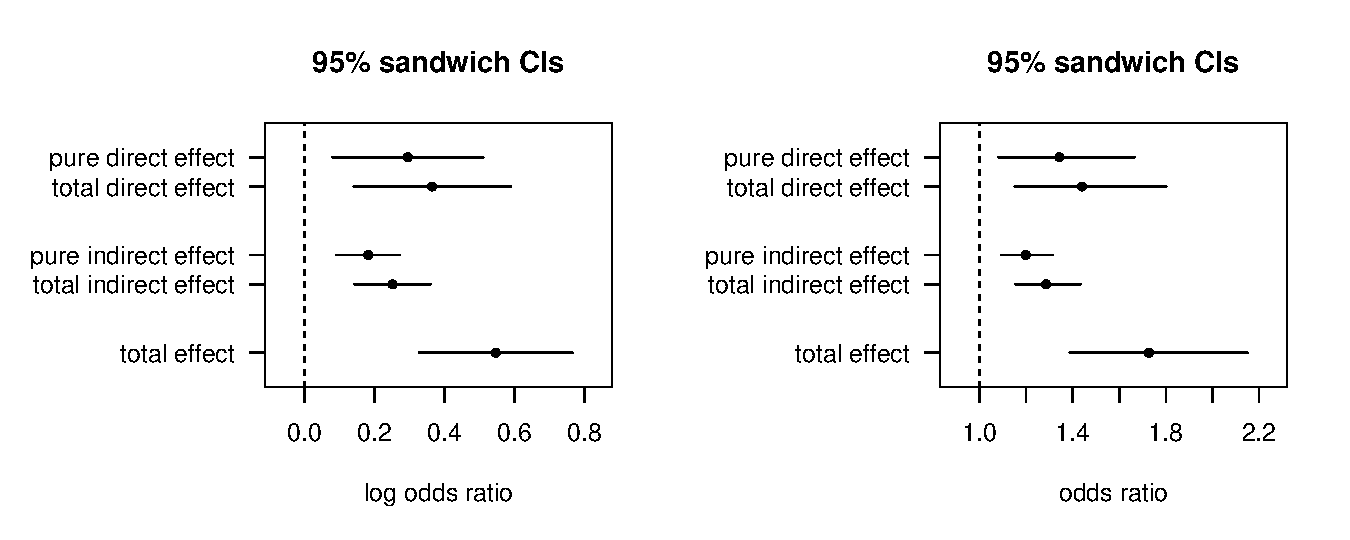
\includegraphics{medflex-fig2}
\end{center}
\vspace{-0.8cm}
\caption{Effect decomposition on the log odds ratio and odds ratio scales.\label{plot-effdecomp}}
\end{figure}
\par Applying the \code{plot} function to a natural effect model object automatically retains the causal effect estimates of interest, generates a linear hypothesis object using \code{neEffdecomp} and then plots its corresponding estimates and confidence intervals, as shown in Figure~\ref{plot-effdecomp}.
\begin{Schunk}
\begin{Sinput}
R> par(mfrow = c(1, 2))
R> plot(neMod2, xlab = "log odds ratio")
R> plot(neMod2, xlab = "odds ratio", transf = exp)
\end{Sinput}
\end{Schunk}
\par The default exposure reference and covariate levels for these plots are the same as for the \code{neEffdecomp} function, but can again be altered via the corresponding arguments \code{xRef} and \code{covLev}.

\section{Population-average natural effects}\label{popavg}
In all previous sections, we defined natural effects as conditional or stratum-specific effects (i.e., conditional on baseline covariates). However, the \pkg{medflex} package additionally allows to estimate population-average natural effects. As demonstrated in Appendix~\ref{app:wweightest} and~\ref{app:wimpest}, rewriting the mediation formula reveals that estimation of these population-average effects requires weighting by the reciprocal of the conditional exposure density in order to adjust for confounding \citep[also see][]{Albert2012a, Vansteelandt2012f}.
\par As a consequence, a model for the exposure density needs to be fitted and specified as an additional working model, e.g.,
\begin{Schunk}
\begin{Sinput}
R> expFit <- glm(att ~ gender + educ + age, data = UPBdata)
\end{Sinput}
\end{Schunk}
Since specifying population-average natural effect models using the \code{neModel} is equivalent for the weighting- and imputation-based approaches, in the remainder of this section, we demonstrate how to proceed when adhering to the imputation-based approach. Moreover, when estimating population-average natural effects, incoherence between imputation and natural effect models is less of a concern as the latter does not require modeling the relation between outcome and covariates. The (first) working model can again be fitted using the same commands as before:
\begin{Schunk}
\begin{Sinput}
R> impData <- neImpute(UPB ~ att + negaff + gender + educ + age,
+    family = binomial("logit"), data = UPBdata)
\end{Sinput}
\end{Schunk}
Each observation in the expanded dataset to which the marginal natural effect model
\begin{align}\label{eq:nemodelweighted}
\mbox{logit} \Pr\left\{Y(x,M(x^*))=1\right\} = \theta_0 + \theta_1 x + \theta_2 x^*
\end{align}
is fitted, needs to be weighted by the reciprocal of the exposure probability density, $\Pr(X|C)$, evaluated at the observed exposure. The fitted model object that is used to calculate regression weights needs to be specified in the \code{xFit} argument of the \code{neModel} function:
\begin{Schunk}
\begin{Sinput}
R> neMod5 <- neModel(UPB ~ att0 + att1, family = binomial("logit"),
+    expData = impData, xFit = expFit, se = "robust")
R> summary(neMod5)
\end{Sinput}
\begin{Soutput}
Natural effect model
with robust standard errors based on the sandwich estimator
---
Exposure: att 
Mediator(s): negaff 
---
Parameter estimates:
            Estimate Std. Error z value Pr(>|z|)    
(Intercept)  -0.5793     0.1112   -5.21  1.9e-07 ***
att0          0.2967     0.1082    2.74   0.0061 ** 
att1          0.2294     0.0578    3.97  7.2e-05 ***
---
Signif. codes:  0 '***' 0.001 '**' 0.01 '*' 0.05 '.' 0.1 ' ' 1
\end{Soutput}
\end{Schunk}

\par Both the marginal natural direct and indirect effect odds ratios again seem to be significantly different from 1: increasing the anxious attachment level from average to one standard error above average, while keeping negative affectivity fixed at levels corresponding to anxious attachment level $x^*$, increases the odds of displaying unwanted pursuit behaviors with a factor
\begin{align*}
\widehat{\mbox{OR}}^{\text{NDE}}_{1,0} &= \frac{\mbox{odds}\left\{Y(1,M(x^*))=1\right\}}{\mbox{odds}\left\{Y(0,M(x^*))=1\right\}} = \exp(\hat{\theta}_1) = 1.35.
\end{align*}
A similar interpretation can again be made for the natural indirect effect.

\section{Intermediate confounding: A joint mediation approach}\label{multmed}
In many settings multiple mediators may be of interest. In our example, one could argue that being anxiously attached to one's partner makes respondents more hesitant to end their relationship and that, in turn, not having initiated the break-up causes them to engage in unwanted pursuit behaviors more often. Initiator status (\code{initiator}: either \code{"both"}, \code{"ex-partner"}, or \code{"myself"}) can thus also be considered a mediator, which we denote $L$.
\par If hypothesized mediators are conditionally independent (given exposure and baseline covariates), separate natural effect models can be fitted (each with a different working model involving only one of the mediators) to assess the mediated effects through each of the mediators one at a time. Specifically, if the aforementioned ignorability conditions \ref{A1}-\ref{A4} hold with respect to each mediator separately\footnote{In addition to the assumptions expressed in \ref{A1}-\ref{A4}, we additionally assume that $Y(x,l) \cip X \vert C$ (for all levels of $x$ and $l$), $L(x) \cip X \vert C$ (for all levels of $x$), $Y(x,l) \cip L \vert X=x,C$ (for all levels of $x$ and $l$) and $Y(x,l) \cip L(x^*) \vert C$ (for all levels of $x$, $x^*$ and $l$).}, natural indirect effects, as defined as causal pathways through single mediators, are identified since these conditions imply that the given mediators are independent given exposure and baseline covariates \citep{Imai2013, VanderWeele2013b}. Recently, \cite{Lange2013a} demonstrated how independent intermediate pathways can be assessed in a single natural effect model using the weighting-based approach. Additionally, these authors proposed a regression-based approach for testing conditional dependence between mediators \citep[also see][]{Loeys2013a, Imai2013}.
\par Often, however, mediators are interdependent and can be thought of as being linked in a sequential causal chain. For instance, not having initiated the break-up could have made respondents more prone to feeling sad, jealous, angry, frustrated or hurt, as reflected in the causal diagram of Figure~\ref{dag2}. Under this diagram, initiator status confounds the relation between the mediator and outcome (given that negative affectivity is the mediator of interest), while at the same time being affected by the exposure, hence violating identification assumption \ref{A4}. As a consequence, the natural indirect effect via negative affectivity is no longer identified under the NPSEM-IE depicted in Figure~\ref{dag2} \citep[although see][for additional (parametric) restrictions which enable identification]{Robins2003, TchetgenTchetgen2014a,Vansteelandt2012d}. This non-identification can intuitively be appreciated by the fact that, in the presence of an intermediate confounder $L$, the natural indirect effect via $M$ can be rewritten as 
\begin{align*}
\frac{\mbox{odds}\left\{Y(x,L(x),M(1,L(1)))=1\vert C\right\}}{\mbox{odds}\left\{Y(x,L(x),M(0,L(0)))=1\vert C\right\}},
\end{align*}
which involves blocking the causal path through $L$ only ($X \rightarrow L \rightarrow Y$), while at the same time assessing the effect transmitted through $L$ and $M$ ($X \rightarrow L \rightarrow M \rightarrow Y$) \citep{Didelez2006}.
\begin{figure}[t]
  \small
  \centering
  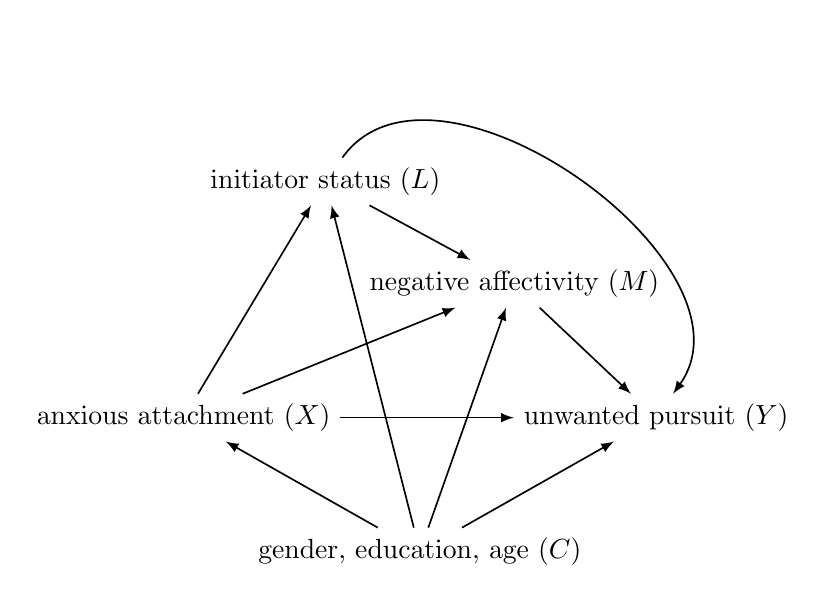
\begin{tikzpicture}[>=latex,semithick]
\node[] (x) at (0, 0)   {anxious attachment ($X$)};
\node[] (l) at (1.8, 3) {initiator status ($L$)};
\node[] (m) at (4.2, 1.7)   {negative affectivity ($M$)};
\node[] (y) at (6, 0)   {unwanted pursuit ($Y$)};
\node[] (c) at (3, -1.7) {gender, education, age ($C$)};
\path[->] (c) edge node [above left] {} (x);
\path[->] (c) edge node [above left] {} (l);
\path[->] (c) edge node [above left] {} (m);
\path[->] (c) edge node [above left] {} (y);
\path[->] (x) edge node [above left] {} (m);
\path[->] (x) edge node [above left] {} (l);
\path[->] (l) edge node [above right] {} (m);
\path[->] (l) edge [bend left=90] node [above right] {} (y);
\path[->] (m) edge node [above right] {} (y);
\path[->] (x) edge node [above right] {} (y);
  \end{tikzpicture}
  \caption{Causal diagram reflecting exposure-induced confounding. \label{dag2}}
\end{figure} 
\par Alternatively, the total causal effect can be decomposed into the effect transmitted through $L$ and $M$ simultaneously and the effect not mediated by any of the given mediators \citep{VanderWeele2013b, VanderWeele2014}. Although such a joint mediation approach might not target the initial mediation hypothesis, it may still shed some light on the underlying causal mechanisms if there are reasons (either theoretical or empirical) to question the validity of condition \ref{A4} (with respect to a single mediator)\footnote{In particular, it can be interesting to assess if the two mediators in combination lead to a null direct effect as this may signal that all important components in the causal chain from exposure to outcome have been identified.}, since this decomposition relies on a weaker set of ignorability assumptions. Specifically, if, as under the NPSEM-IE depicted in Figure~\ref{dag2}, we assume that a set of baseline covariates $C$ satisfies `no omitted variables' assumptions \ref{A1}-\ref{A3} with respect to $L$ and $M$ jointly (rather than separately) and that no measured or unmeasured confounders of the $(L,M)-Y$ relation are affected by the exposure\footnote{I.e., assuming that $Y(x,l,m) \cip X \vert C$ (for all levels of $x$, $l$ and $m$), $\{M(x), L(x)\} \cip X \vert C$ (for all levels of $x$), $Y(x,l,m) \cip \{L,M\} \vert X=x,C$ (for all levels of $x$, $l$ and $m$) and $Y(x,l,m) \cip \{L(x^*),M(x^*)\} \vert C$ (for all levels of $x$, $x^*$, $l$ and $m$).}, the joint mediated effect and corresponding direct effect are identified. The appeal of this joint mediation approach is that by defining a natural indirect effect with respect to a set or vector of mediators (rather than a single mediator) assumption \ref{A4} can be made more plausible by simply including mediator-outcome confounders that are deemed likely to be affected by the exposure in the joint set of mediators \citep{VanderWeele2013b}.
\par For example, $\exp(\beta_1^{\star\star})$ in model~\eqref{eq:nemodelmultiv}
\begin{align}
\mbox{logit} \Pr\left\{Y(x,L(x^*),M(x^*, L(x^*)))=1|C\right\} = \beta_0^{\star\star} + \beta_1^{\star\star} x + \beta_2^{\star\star} x^* + \beta_3^{\star\star} C,
\label{eq:nemodelmultiv}
\end{align}
captures the (newly defined) natural direct effect odds ratio 
$$
\mbox{OR}^{\text{NDE}}_{1,0|C} = \frac{\mbox{odds}\left\{Y(1,L(x^*),M(x^*, L(x^*)))=1|C\right\}}{\mbox{odds}\left\{Y(0,L(x^*),M(x^*, L(x^*)))=1|C\right\}},
$$
whereas $\exp(\beta_2^{\star\star})$ captures the natural indirect effect odds ratio
$$
\mbox{OR}^{\text{NIE}}_{1,0|C} = \frac{\mbox{odds}\left\{Y(x,L(1),M(1, L(1)))=1|C\right\}}{\mbox{odds}\left\{Y(x,L(0),M(0, L(0)))=1|C\right\}}
$$ 
through $L$ and $M$ jointly.
\par Fitting this natural effect model, however, requires both mediators to be taken into account in the working model(s). When applying the weighting-based approach, dealing with multiple mediators entails fitting a model for each of the mediators separately to calculate ratio-of-mediator probability weights, as in \cite{Lange2013a}. The imputation-based approach, on the other hand, is less demanding as it only requires one working model for the outcome. For this reason, estimation of joint mediated effects is implemented only for the imputation-based approach in the current version of the \pkg{medflex} package.
\par Hence, after expanding the data, nested counterfactual outcomes need to be imputed by fitted values from an imputation model conditional on both $L$ and $M$. For instance, in the \proglang{R} code below, a logistic model
\begin{align*}
\mbox{logit} \Pr(Y=1|X,L,M,C) = \gamma^{\star\star}_0 + \gamma^{\star\star}_1 X + \gamma^{\star\star}_2 L + \gamma^{\star\star}_3 M + \gamma^{\star\star}_4 LM + \gamma^{\star\star}_5 C
\end{align*}
is fitted that allows the mediators to interact in their effect on the outcome.
\begin{Schunk}
\begin{Sinput}
R> impData <- neImpute(UPB ~ att + initiator * negaff + gender + educ + age,
+    family = binomial("logit"), nMed = 2, data = UPBdata)
\end{Sinput}
\end{Schunk}
The number of mediators to be considered jointly should be set via the \code{nMed} argument in the \code{neImpute} function. If \code{nMed = 2}, not only the second predictor variable, but the two predictor variables declared after the exposure variable are internally coded as mediators. Subsequently, natural effect model~\eqref{eq:nemodelmultiv} can be fitted to the imputed dataset using the \code{neModel} function.
\begin{Schunk}
\begin{Sinput}
R> neMod6 <- neModel(UPB ~ att0 + att1 + gender + educ + age,
+    family = binomial("logit"), expData = impData, se = "robust")
R> summary(neMod6)
\end{Sinput}
\begin{Soutput}
Natural effect model
with robust standard errors based on the sandwich estimator
---
Exposure: att 
Mediator(s): initiator, negaff 
---
Parameter estimates:
            Estimate Std. Error z value Pr(>|z|)    
(Intercept)  -0.4919     0.6854   -0.72    0.473    
att0          0.2444     0.1114    2.19    0.028 *  
att1          0.2476     0.0538    4.60  4.2e-06 ***
genderM       0.2629     0.2274    1.16    0.248    
educM         0.2780     0.4912    0.57    0.571    
educH         0.4223     0.4979    0.85    0.396    
age          -0.0121     0.0122   -0.99    0.320    
---
Signif. codes:  0 '***' 0.001 '**' 0.01 '*' 0.05 '.' 0.1 ' ' 1
\end{Soutput}
\end{Schunk}
Correct specification of the (number of) mediators can easily be checked in the \code{summary} output of the natural effect model object, which lists the names of the exposure and all mediators. 
\par Although we have hypothesized that initiator status affects the level of experienced negative affectivity, this joint mediator approach does not necessarily require knowing the ordering of the mediators. \cite{VanderWeele2013b} and \cite{VanderWeele2014} described how additional insight into the causal mechanisms can be gained when the ordering is (assumed to be) known. These authors advocated a sequential approach which enables further effect decomposition of the total causal effect into multiple path-specific effects (\citealt{Avin2005}; also see \citealt{Huber2013} for an inverse-probability weighting approach and \citealt{Albert2011} and \citealt{Daniel2015} for a parametric g-computation approach for estimating some of these path-specific effects). Such sequential approach can easily be embedded in the natural effect model framework and is planned to be implemented in an upcoming version of the \pkg{medflex} package.

\section{Weighting or imputing?}\label{weightimp}
For both the weighting- and imputation-based approach, valid estimation of natural effects hinges on adequate specification of their corresponding nuisance working models and the natural effect model. In this section, we highlight the impact of model misspecification for each of the two proposed estimation approaches. The resulting trade-off in terms of modeling demands may serve as a guideline as to which of the two approaches is to be preferred in which particular setting. Moreover, certain missing data patterns might also favor one approach over the other, as discussed in more detail below.

\subsection{Modeling demands}
The proposed weighting-based approach yields consistent natural effects estimates if both the natural effect model and the conditional distribution of the mediator are correctly specified. The latter needs careful consideration, especially when exposure or baseline covariates are highly predictive of the mediator, for then even minor misspecifications in its conditional expectation can have a major impact on the weights and lead to heavily biased estimation of the target natural effects parameters. However, residual plots with scatterplot smoothers are often helpful to diagnose model inadequacy and can be requested, for instance, by passing the \code{expData}-class object to the \code{residualPlots} function from the \pkg{car} package. When dealing with continuous mediators, correct modeling not only demands adequate specification of the mediator's expectation, but also requires additional parametric assumptions on the mediator's conditional density (i.e., the distribution of the error terms).\footnote{By default, the density function will correspond to the error distribution specified in the \code{family} argument for the mediator model (in turn specified via \code{neWeight}). QQ plots of the residuals can in this case be informative as to whether this parametric assumption is warranted for continuous mediators and can be obtained using the \code{qqnorm} function. The residuals can easily be obtained directly from the expanded dataset (as the working model is stored as an attribute in the expanded dataset object) by the command \code{residuals(expData)}.} Moreover, even under proper model specification, weights for continuous mediators typically tend to be unstable, leading to less precise natural effect estimates and considerable finite sample bias. In particular, when the outcome is linear in the mediator, it might be sensible to avoid unnecessary parametric assumptions, since then the mediation formula prescribes only correct specification of the mediator's expectation.
\par In the light of these considerations, \cite{Vansteelandt2012} recommended routine application of the imputation-based approach, especially when dealing with continuous mediators, since it avoids reliance on a model for the mediator. Despite this attraction, the imputation estimator does not come without limitations.
\par As in other imputation settings, one must pay due attention to coherent (or `congenial') specification of the imputer's model and the analyst's model (i.e., in this case, the natural effect model) \citep{Meng1994}. This might be particularly challenging for nonlinear outcome models. For instance, when using logistic regression to model binary outcomes, the imputation model may be difficult or impossible to match with the natural effect model \citep{VanderWeele2010, TchetgenTchetgen2014}. To limit the impact of potential model uncongeniality in terms of misspecification bias, \cite{Vansteelandt2012} and \cite{Loeys2013a} advocated the use of a sufficiently rich imputation model.\footnote{A `minimal' imputation model should thus at least reflect the structure of the natural effect model (e.g., also including exposure-mediator interactions when these are postulated in the natural effect model as an interaction term between $x$ and $x^*$) to avoid attenuation of the estimates of effects that were precluded from the imputation model.} To this end, the \pkg{medflex} package allows users to fit an imputation model using generalized additive models or machine learning techniques, such as the ensemble learner as implemented in the \pkg{SuperLearner} package \citep{R:SuperLearner}.\footnote{An example is given in the help files of the package and can be consulted via \code{?neImpute.default}. Only bootstrap standard errors are available when fitting the imputation model using the \code{SuperLearner} function.} Moreover, issues of uncongeniality can be avoided altogether by resorting to saturated natural effect models. In practice, models for conditional natural effects will rarely be saturated as either (some) baseline covariates or the exposure variable are continuous (or both). If the exposure is categorical, saturated models can be fitted for estimating population-average rather than stratum-specific natural effects (see Section~\ref{popavg}). However, for observational data, as opposed to data from experiments where the exposure is randomly assigned, adjustment for confounding in population-average natural effect models requires inverse weighting for the exposure.\footnote{Note that in both settings all baseline confounders still need to be adjusted for in the imputation model. Moreover, although the use of population-average natural effect models can, in some settings, avoid issues concerning potential model uncongeniality, it is up to the researcher to decide whether stratum-specific or population-average effects are the target of the study.}
\par Second, as opposed to the weighting-based estimator, estimation by imputation requires modeling the mediator-outcome relation, which can be far from trivial whenever the exposure or baseline covariates are strongly associated with the mediator. In these scenarios, information about the effect of the mediator on the outcome may be sparse within certain strata defined by the exposure and covariates and, as a result, model misspecification may be difficult to diagnose and extrapolation bias becomes more likely \citep{Vansteelandt2012f}. Whenever increased concerns of model extrapolation arise, the weighting-based approach may be indicated, as extrapolation uncertainty will typically be more honestly reflected in the corresponding standard errors \citep{Vansteelandt2012a}.\footnote{Extrapolation might also affect estimation in the natural effect model, primarily when baseline covariates and exposure are highly correlated. This concern holds for both the weighting- and imputation-based estimator, since both require regression adjustment for covariates to estimate conditional natural effects.}
\par Finally, it can be argued that, for both estimation approaches, if the working model is correctly specified (either via generalized linear models or via more advanced techniques), a parsimonious (and possibly misspecified) natural effect model will still provide some summary result tailored to answer the practitioner's main research questions \citep{Vansteelandt2012, Loeys2013a}. Suppose, for instance, that the logistic regression models in equation~\eqref{0} are correctly specified. Fitting a natural effect model of the form
\begin{align*}
\mbox{logit} \Pr(Y=1|X,M,C) = \beta_0 + \beta_1 x + \beta_2 x^* + \beta_3 C
\end{align*}
to the expanded dataset using the imputation-based approach will then yield an estimated conditional natural indirect effect odds ratio of 1.143, which can be roughly considered as the mean conditional odds ratio across potential exposure levels (as depicted in Figure~\ref{ill}). If such an approach turns out to be unsatisfactory, users can again request residual plots to guide further model building and improve goodness-of-fit (by calling the \code{residualPlots} function). These diagnostics can be particularly helpful in the presence of certain non-linearities. For instance, when a continuous mediator is quadratic in the exposure, residual plots will indicate the need for a quadratic term for the indirect effect in the natural effect model, which will usually go unnoticed when fitting an imputation model for the outcome. 

\subsection{Missing data}
As previously stated, when missingness occurs in the outcome, this is naturally dealt with when choosing the imputation-based approach, as missing outcomes in the original dataset are (by default) imputed in the expanded dataset, under the assumption that these outcomes are MAR (missing at random) given exposure, mediator(s) and baseline covariates.\footnote{It might be necessary to include additional covariates (that are both predictive of the outcome and missingness in the outcome, but are not included in the set of baseline covariates, $C$, that is chosen to meet assumptions \ref{A1}-\ref{A4} to the imputation model to make the MAR assumption more plausible.} 
\par The weighting-based approach, on the other hand, is restricted to the analysis of complete cases and hence requires the more stringent MCAR (missing completely at random) assumption to hold in order to obtain unbiased estimation of the natural effect parameters. Whenever missingness occurs only in the outcome, we therefore advise to use the imputation-based approach. Alternatively, one might resort to multiple imputation, as also recommended if missingness occurs in either the exposure, mediator(s) or baseline covariates. 
\par For instance, the \code{mice} function from the \pkg{mice} package \citep{R:mice} can be used to obtain multiply imputed datasets (stored in a \code{mids}-class object). The working model can in turn be fitted to each of these datasets by passing them (or rather the object containing these datasets) to the \code{with.mids} function, which also processes the function (i.e., either \code{neWeight} or \code{neImpute}) and expression that needs to be evaluated via the second argument. These steps are illustrated in the code below, in which \code{missdat} is a copy of the UPB dataset with artificially introduced missingness in each of the original variables.
\begin{Schunk}
\begin{Sinput}
R> library("mice")
R> library("mitools")
R> 
R> missdat <- UPBdata
R> for (i in 1:ncol(missdat)) {
+    missdat[sample(nrow(missdat))[1:10], i] <- NA
+  }
R> 
R> multImp <- mice(missdat, m = 10)
R> expData <- with(multImp, neWeight(negaff ~ factor(attbin) + gender 
+    + educ + age))
\end{Sinput}
\end{Schunk}
Next, we use some functionalities from the \pkg{mitools} package \citep{R:mitools} to fit natural effect model~\eqref{eq:nemodelnoia} to each of the expanded multiply imputed datasets (stored in \code{expData$analyses}). The function \code{imputationList} can be used to transform the output containing these expanded datasets into a format that can be further passed to the \code{with.imputationList} function.
\begin{Schunk}
\begin{Sinput}
R> expData <- imputationList(expData$analyses)
R> neMod1 <- with(expData, neModel(UPB ~ attbin0 + attbin1 + gender 
+    + educ + age, family = binomial("logit"), se = "robust"))
\end{Sinput}
\end{Schunk}
Finally, the results can be pooled by using the \code{MIcombine} function.
\begin{Schunk}
\begin{Sinput}
R> MIcombine(neMod1)
\end{Sinput}
\begin{Soutput}
Multiple imputation results:
      with(expData, neModel(UPB ~ attbin0 + attbin1 + gender + educ + 
    age, family = binomial("logit"), se = "robust"))
      MIcombine.default(neMod1)
                results         se
(Intercept) -0.84709412 0.73366115
attbin01     0.37963076 0.21874683
attbin11     0.34933687 0.08987945
gender2      0.34072605 0.24124907
educ2        0.14410803 0.49349023
educ3        0.39779433 0.50418124
age         -0.01097623 0.01299724
\end{Soutput}
\end{Schunk}

\section[Concluding remarks]{Concluding remarks}\label{concl}
In this paper, we provided some theoretical background on the counterfactual framework, in particular on mediation analysis and natural direct and indirect effects, and described the functionalities of the \proglang{R} package \pkg{medflex}. 
\par This package combines some important strengths of other (software) applications for mediation analysis that build on the mediation formula, while accommodating some of their respective weaknesses. The major appeal of this package is its flexibility in dealing with nonlinear parametric models and the functionalities it offers for hypothesis testing by resorting to natural effect models, which allow for direct parameterization of the target causal estimands on their most natural scale. Furthermore, for the most common parametric models, robust standard errors can be obtained, so the computer-intensive bootstrap can be avoided. A limitation of this package is that, at present, it does not offer any tools for assessing the sensitivity of one's results to possible violations of the identification assumptions of the causal estimands.
\par As mentioned in section~\ref{multmed}, additional functionalities for dealing with exposure-induced confounding and multiple mediators are intended to be added to the package in the future, as well as extensions for survival models. Future developments within the realm of natural effect models (such as a generic framework for conducting sensitivity analyses) will be added in updates of the package.

\appendix

\section[]{Link between estimators and the mediation formula}
In this section we illustrate in more detail how natural effect models can be regarded as alternative formulations of the mediation formula.
\subsection[]{Weighting-based estimator \citep{Lange2012}}\label{app:weightest}
Fitting a stratum-specific natural effect model using the weighting-based approach requires a model for the mediator distribution $\Pr(M|X,C)$ as a working model.
\begin{fleqn}
\begin{align*}
\E\left\{Y(x,M(x^*))|C\right\} &= \sum_m \E(Y|X=x,M=m,C) \Pr(M=m|X=x^*,C)\\[5pt]
&= \sum_y \sum_m y \Pr(Y=y|X=x,M=m,C) \Pr(M=m|X=x^*,C)\\[5pt]
&= \sum_y \sum_m y \dfrac{\Pr(Y=y,M=m|X=x,C)}{\Pr(M=m|X=x,C)} \Pr(M=m|X=x^*,C)\\[5pt]
&= \E\left[\ Y \dfrac{\Pr(M=m|X=x^*,C)}{\Pr(M=m|X=x,C)} \ \middle\vert \ X=x,C
\ \right]
\end{align*}

\subsection[]{Imputation-based estimator \citep{Vansteelandt2012}}\label{app:impest}
Fitting a stratum-specific natural effect model using the imputation-based approach requires an imputation model for the mean outcome $\E(Y|X,M,C)$ as a working model.
\begin{align*}
\E\left\{Y(x,M(x^*))|C\right\} &= \sum_m \E(Y|X=x,M=m,C) \Pr(M=m|X=x^*,C) \nonumber\\
&= \E\Big[\ \E(Y|X=x,M,C) \ \Big\vert \ X=x^*,C
\ \Big]
\end{align*}

\subsection[]{Weighted weighting-based estimator \citep{Lange2012}}\label{app:wweightest}
Fitting a marginal or population-averaged natural effect model requires a propensity score model for the exposure $\Pr(X|C)$ as additional working model.
\begin{align*}
\E\{Y(x,M(x^*))\} &= \sum_c \sum_m \E(Y|X=x,M=m,C=c) \Pr(M=m|X=x^*,C=c) \Pr(C=c)\\[5pt]
&= \sum_y \sum_c \sum_m  y \Pr(Y=y|X=x,M=m,C=c)\\[-10pt] & \qquad \qquad \qquad {} \times \Pr(M=m|X=x^*,C=c) \dfrac{\Pr(C=c, X = x)}{\Pr(X = x \vert C=c)}\\[5pt]
&= \sum_y \sum_c \sum_m y \dfrac{\Pr(Y=y,M=m|X=x,C=c)}{\Pr(M=m|X=x,C=c)}\\[-5pt] & \qquad \qquad \qquad {} \times \Pr(M=m|X=x^*,C=c) \dfrac{\Pr(C=c, X = x)}{\Pr(X = x \vert C=c)}\\[5pt]
&= \sum_y \sum_c \sum_m y \dfrac{\Pr(Y=y,M=m,C=c,X=x)}{\Pr(X = x \vert C=c)} \dfrac{\Pr(M=m|X=x^*,C=c)}{\Pr(M=m|X=x,C=c)}\\[5pt]
&= \sum_y \sum_c \sum_m y \dfrac{\Pr(Y=y,M=m,C=c\vert X=x)}{\Pr(X = x \vert C=c)} \Pr(X=x)\\[0pt] & \qquad \qquad \qquad {} \times \dfrac{\Pr(M=m|X=x^*,C=c)}{\Pr(M=m|X=x,C=c)} \\[5pt]
&= \E\biggl[\dfrac{Y}{\Pr(X = x \vert C)} \dfrac{\Pr(M|X=x^*,C)}{\Pr(M|X=x,C)} \bigg\vert\ X=x \biggr] \Pr(X=x)\\[5pt]
&= \E\biggl[\dfrac{Y I(X=x)}{\Pr(X = x \vert C)} \dfrac{\Pr(M|X=x^*,C)}{\Pr(M|X=x,C)} \biggr]
\end{align*}

\subsection[]{Weighted imputation-based estimator \citep[related to][]{Albert2012a}}\label{app:wimpest}
\begin{align*}
\E\{Y(x,M(x^*))\} &= \sum_c \sum_m \E(Y|X=x,M=m,C=c) \Pr(M=m|X=x^*,C=c) \Pr(C=c)\\[5pt]
&= \sum_c \sum_m \dfrac{\E(Y|X=x,M=m,C=c)}{\Pr(X = x^* \vert C=c)} \Pr(M=m,C=c,X=x^*)\\[5pt]
&= \sum_c \sum_m \dfrac{\E(Y|X=x,M=m,C=c)}{\Pr(X = x^* \vert C=c)} \Pr(M=m,C=c\vert X=x^*) \Pr(X = x^*)\\[5pt]
&= \E\left[\
\dfrac{\E(Y|X=x,M,C)}{\Pr(X=x^*|C)}
\ \middle\vert\ X=x^*
\ \right] \Pr(X = x^*)\\[5pt]
&= \E\left[\dfrac{\E(Y|X=x,M,C)}{\Pr(X=x^*|C)}  I(X=x^*)\right]
\end{align*}
\end{fleqn}

\bibliography{bib}
\newpage
\end{document}
